\newcommand\T{\rule{0pt}{2.6ex}}
\newcommand\B{\rule[-1.2ex]{0pt}{0pt}}
\newcommand{\dndeta}{\ensuremath{\mathrm{d}N_{\rm ch}/\mathrm{d}\eta}}
\newcommand{\micro}{\ensuremath{\mu}}

\newcommand*\andnewline{%
        \end{tabular}
        \\[\bigskipamount]
        \begin{tabular}[t]{c}
}
\section{Simulating radiation effects in silicon sensors and modelling charge response}
\label{sec:sensorsim}
{\it Editors: M.~Bomben, J.~Sonneveld}  \\
{\it Contributing authors: A.~Alici, M.~Benoit, M.~Bomben, E.~Chabert, A.~Di~Mauro, J.~Merino, B.~Nachman, L.~Rossini, P.~Sabatini, J.~Sonneveld, C.~Suarez, M.~Swartz, T.~Szumlak, A.~Wang}  \\

\noindent
Simulating radiation damage is critical in order to make accurate predictions of the performance of the detector, that will enable searches for new particles and forces as well as precision measurements of Standard Model particles. In what 
follows the strategies implemented by the LHC experiments to correctly simulate the evolution  of silicon tracking detectors performance with luminosity
 will be presented. \\
As already said in this report's introduction the main macroscopic
 effects on silicon tracking devices due to radiation damage are: 
increase of leakage current, change of operational voltage and signal loss. They are the consequence of phenomena 
happening at microscopic level, due to the creation of bulk defects which act as deep levels in the energy gap. These 
levels can charge up by trapping carriers and act as additional generation levels: these dynamics directly relate to the
aforementioned change in performance at macroscopic level. \\
Thus the general parameterisation of radiation damage simulation for silicon tracking detectors of LHC experiments  has to model 
the change  of the electric field distribution in the silicon bulk  and 
the signal loss with the accumulated luminosity. These two effects will affect also other observables as for example the spatial resolution, through 
modification of cluster sizes and Lorentz Angle deflection. \\
Before presenting the details and results of the different LHC experiments some general aspects of the simulations 
are discussed.

\noindent
\textbf{Model of signal digitization}
In detector simulation the drift of electron-hole pairs produced by crossing charged particles travels towards the electrodes and the consequent charge induction on electrodes is the so-called \textit{digitization} step.\\
\noindent
\textbf{Electric field} Due to radiation damage the shape of the electric field inside the bulk of the sensor changes depending on the fluence. Simulations of the three-dimensional profile of the electric field can be obtained with software based on technology computer-aided design (TCAD).\\
% explain tcad
%TCAD \cite{tcadref} is \dots
\noindent
\textbf{Lorentz angle}
The Lorentz angle ($\theta_L$) is defined as the angle between the drift direction and the electric field. This is due to the presence of the magnetic field $\vec{B}$. 
For a carrier travelling from an initial bulk depth $z_i$\footnote{when referring to silicon sensors the local coordinate $z$ identifies the direction orthogonal to the collecting electrodes in planar technology and the one parallel to the columns axis in 3D technology} to a final one $z_f$ inside the bulk 
of the sensor the Lorentz Angle $\theta_L$ can be expressed by:
\begin{equation}
\tan\theta_L (z_i,z_f) = \frac{rB}{|z_f - z_i |}\int^{z_f}_{z_i}\mu(E(z))dz,
\label{eq:LA}
\end{equation}
where $\mu$ is the mobility, $r$ is the Hall scattering factor, $B$ is the magnetic field magnitude, and $E(z)$ is the electric field as a function of the position. It is then possible to note that a change in electric field due to the radiation damage will impact also the Lorentz Angle, since the mobility depends on the electric field.\\

\noindent
\textbf{Charge Trapping}
The charge carriers can be trapped by radiation induced deep defects, with a characteristic
trapping time $\tau$ 
that is proportional to the inverse of the radiation fluence $\Phi$: $\tau = 1/(\Phi\beta)$, where $\beta$ is the trapping constant. \\

\noindent
\textbf{Ramo potential and induced charge}
%Drifting charges inside the bulk of the sensors towards the electrodes induce a signal that is then read by the electronics. 
Moving charges inside the bulk induce a signal onto collecting electrodes. The  induced signal   can be 
calculated using the Shockley-Ramo theorem \cite{Ramo}. %This is estimated as,
The induced signal by a charge $q$ moving from the initial position $\vec{x}_i$ to the final position $\vec{x}_f$ is:
\begin{equation}
Q_{\text{induced}} = -q[\phi_{\text{w}}(\vec{x}_{\text{f}})-\phi_{\text{w}}(\vec{x}_{\text{i}})],
\label{eq:ramopotential}
\end{equation}
where $\phi_{\text{w}}$ is the Ramo potential. The Ramo potential depends only on the geometry of the electrodes and the bulk thickness, and therefore it is evaluated once per geometry.\\

\noindent
\textbf{Charge Collection Efficiency}
One important observable to monitor is the collected charge, which is reported as the most probable value of the cluster charge  distribution. The charge collection efficiency (CCE) is defined as the ratio of the most probable value of the cluster charge distribution of a certain point against the value  before  irradiation. The evolution of CCE with luminosity is important 
to determine the sensor operational voltage: simulations of CCE vs bias voltage for different radiation fluences are 
used to assure that the detector is collecting the largest possible amount of signal.\\

\noindent In Figure~\ref{digitizer_diagram} a schematic view of the process flow presented above.
\begin{figure}[htbp]
\begin{center}
\includegraphics[width=0.43\textwidth]{figures/SensorSimulation/digitizer_diagram.pdf}
\caption{An illustration of the digitization process for the planar sensors~\cite{Aaboud:2019wgd}}
\label{digitizer_diagram}
\end{center}
\end{figure}

\noindent
In what follows the simulations implementation of ATLAS~(\ref{sec:ATLAS}), CMS~(\ref{sec:CMS}), 
LHCb~(\ref{sec:LHCb}) and ALICE~(\ref{sec:ALICE}) will be presented. In Section~\ref{sec:Inter-experiment comparisons}  
the different strategies of the LHC experiments will be compared; eventually (Sec.~\ref{sec:discussion_and_outlook}) 
conclusions and outlook will be drawn.


\subsection{ATLAS}
\label{sec:ATLAS}

%\section{The ATLAS Pixel Detector and Radiation Damage effects}
The ATLAS \cite{Aad:2008zzm} Pixel Detector \cite{Aad:pixele} is the innermost component of the Inner Detector\cite{ATLAS:1997ag,ATLAS:1997af}.  As the closest detector component to the interaction point, this detector was subjected to a significant amount of radiation over their lifetime.
%Simulating radiation damage is then critical in order to make accurate predictions of the performance of the detector,  that will enable searches for new particles and forces as well as precision measurements of Standard Model particles.\\
Of the four barrel layers of the Pixel detector, the IBL is the closest one to the beam pipe\footnote{ATLAS uses a right-handed coordinate system with its origin at the nominal interaction point (IP) in the centre of the detector and the $z$-axis coinciding with the axis of the beam pipe. The $x$-axis points from the IP towards the centre of the LHC ring, and the $y$-axis points upward. Cylindrical coordinates $(r, \phi)$ are used in the transverse plane, $\phi$  being the azimuthal angle around the $z$-axis. The pseudorapidity is defined in terms of the polar angle $\theta$ as $\eta = \ln \tan(\theta/2)$.}. The total fluence received during its lifetime has been of $\sim 1 \times 10^{15}\,  n_{\textrm{eq}}/\textrm{cm}^2$ at the end of Run 2 (corresponding to a luminosity delivered by the LHC of 159 fb$^{-1}$), while a total fluence of $1.8\times 10^{15}\,  n_{\textrm{eq}}/\textrm{cm}^2$ is estimated by the end of Run 3 in 2023 (with a total estimated integrated luminosity of $300~\ \textrm{fb}^{-1}$). Figure \ref{fig:LumiVsFluence} shows the fluence received by the four barrel layers as a function of the number of days since the start of Run 2 .\\
In what follows the details of a new digitizer that accounts for effects due to radiation damage will be 
repsented. Section \ref{sec:digMod} presents the model used and each component used, and Section \ref{sec:dataval} presents the results of the simulation compared with data from Run2.


\begin{figure}[!htb]
\centering
%\includegraphics[width=0.7\textwidth]{fig_01_2018}
\includegraphics[width=0.45\textwidth]{figures/SensorSimulation/lorentz.png}
\caption{Estimates of the lifetime fluence experienced by the four layers of the current ATLAS pixel detector as a function of time since the start of Run 2 (June 3, 2015) at $z \sim 0$. The IBL curve represents both the fluence on the IBL (left axis) as well as the delivered integrated luminosity in Run 2 (right axis). From Ref. \cite{PixelLumiAndFLuence}.}
\label{fig:LumiVsFluence}
\end{figure}


\subsubsection{ATLAS Pixels Digitizer Model Overview}
\label{sec:digMod}
%Electron-hole pairs produced by crossing charged particles travels towards the electrodes and induce a charge that is converted into digital signal.
%In simulations, this is done in the \textit{digitization} step.
In the digitization step, energy deposits are obtained from Geant4 \cite{GEANT4}, and saved in a list of position and energy, called \textit{hits}. Radiation damage effects are modelled  in this simulation step for ATLAS Pixel sensors. The 
algorithm which will be presented here was first developed on AllPix \cite{software:Allpix}, a Geant4-based tool which allows an easy and fast simulation of silicon detectors performance after radiation damage. Afterwards, the model was also implemented in the ATLAS common software Athena, in order to exploit the full-geometry description of the ATLAS detector, and check what the effects on physical quantities would be. In both cases the structure of the main algorithm to evaluate the effects of the radiation damage is the same. \\
% I'm not sure this is true:
% As a comparison, in CMS the radiation damage effects are implemented as a posteriori correction to the processed signals, based on measurements of radiation damage effects on collision data.
% In CMS, there are corrections at the digitization step for the position of the cluster, as well as after reconstruction to the pulse height measured in the pixels.

The algorithm for simulating radiation damage within the ATLAS Athena digitizer is as follows:

\begin{itemize}
\item{After charge deposition by Geant4, the digitizer takes in as input the charge and position of the various particles, as well as global information such as the electric field profile after radiation damage}
\item{Groups of $O$(10) charges are formed to be treated as a charge chunk to speedup the digitization}
\item{Using the electric field distribution - based on voltage and fluence - the time for the charge chunk to drift to 
the electrode is evaluated}
\item{This drift time is compared to a randomly generated trapping time; the final bulk depth for the chunk is hence determined}
\item{Deflections are calculated evaluating the average LorentzAngle along the path (using Eq.~\ref{eq:LA}) and 
the contribution of thermal diffusion, hence the final charge chunk position is determined}
\item{ Based on the initial and final charge positions the induced charge on the electrode is then determined using the  Ramo potential (Eq.~\ref{eq:ramopotential}) }
\end{itemize}

% \begin{figure}[htbp]
% \begin{center}
% \includegraphics[width=0.43\textwidth]{figures/SensorSimulation/digitizer_diagram.pdf}
% \caption{An illustration of the digitization process for the planar sensors}
% \label{digitizer_diagram}
% \end{center}
% \end{figure}

\paragraph*{Geometry and Conditions Configuration}
The first step of the software consists in the loading of all the geometry and operational parameters needed: thickness, pitch, tilt, fluence, trapping time, temperature, and magnetic field strength. Lookup tables are then loaded for Ramo potential, electric field maps, and Lorentz angle maps.
Geant4 then generates the energy hits and these are converted into electron-hole pairs; the energy needed is  $\sim 3.6\, \textrm{eV}$ for a pair. 
Charges are then drifted towards the electrodes, and using the pre-loaded maps the probability of being trapped is calculated, and then, using the Ramo potential, the induced charge on the electrodes is evaluated. \\
The different inputs to digitization are described in the following paragraphs.


\paragraph*{Fluence}
Fluence is an important input for the simulations, and in order to compare them to data it is needed to know the correct fluence corresponding to the luminosity. This is obtained from the measurement of leakage current compared with the predictions. Figure \ref{fig:FluenceLeak} (left) shows the predicted leakage current compared with data during Run 2. Figure \ref{fig:FluenceLeak} (right) shows the conversion factor from luminosity to fluence for the IBL, as a function of $z$, compared with predictions with Pythia8+FLUKA \cite{Sjostrand:2014zea,Ferrari:898301} and Pythia+Geant4. From a comparison with the different simulation an error of 15 \% is assumed on this conversion factor.


\begin{figure}[!htb]
\centering
%\includegraphics[width=0.7\textwidth]{fig_01_2018}
%\includegraphics[width=0.45\textwidth]{lorentz.png}
\begin{minipage}[t]{0.6\textwidth}
\vspace{0.25cm}
\includegraphics[width=0.9\textwidth]{figures/SensorSimulation/ileak_fig_01.pdf}
\end{minipage}
\begin{minipage}[t]{0.37\textwidth}
\vspace{-0.44cm}
\includegraphics[width=1.\textwidth]{figures/SensorSimulation/arXivversion_fig_03.pdf}
\end{minipage}
\caption{Left: Average measured leakage current data of a representative sample of modules in the ATLAS Pixel Detector barrel layers over the full period of operation. The leakage current data are normalized to 0$^{\circ}$C; the average module sensor temperature is shown in the top panel. From Ref. \cite{PixelLumiAndLeak}. Right: The fluence-to-luminosity conversion factors (extracted from leakage current fits), as a function of $z$, compared with the Pythia+FLUKA and Pythia+Geant4 predictions. From Ref. \cite{Aaboud:2019wgd}.}
\label{fig:FluenceLeak}
\end{figure}


\paragraph*{Electric Field}
%Due to radiation damage the shape of the electric field inside the bulk of the sensor changes depending on the fluence. Simulations of the profile of the electric field are obtained with a software based on TCAD technologies. 
Once the fluence level is known the electric field profile inside the silicon sensors can be 
calculated for different bias voltages using TCAD tools.
The radiation damage models used in TCAD for simulating the electric field profile were the Chiochia model \cite{mod:Chiochia} for planar sensors and the Perugia model \cite{Perugia} for the 3D sensors. The Chiochia model uses a double trap, with one acceptor and one donor trapping center, with energy level at $E_C-0.525$ eV and $E_V+0.48$ eV for the conduction $E_C$ and valence band energy level $E_V$ respectively. Instead in the Perugia model there are instead three trap levels: two acceptor and one donor trap with energies as: $E_C-0.42$ eV, $E_C-0.46$ eV, and $E_V+0.36$ eV. 
As anticipated, in order to save simulation time many quantities derived from the electric field (such as the time for a charge to drift to an electrode) are also precomputed and saved as maps. Further details can be found in \cite{Aaboud_2019}.

%The electric fields for the planar (3D) sensors are computed from TCAD simulations with the Chiochia\cite{CHIOCHIA200651} (Perugia\cite{7542192}) model. 

The two main parameters for generating maps are the fluence and the bias voltage. Typically, the electric field is computed only for a few benchmark pair, but it is of course not feasible to precompute all possible combinations. Recently, a new method has been developed to produce 
electric field maps for any (fluence, voltage) pair on the fly within the digitizer by interpolating existing electric field maps. This takes advantage of the fact that the electric field at a fixed sensor depth varies smoothly with fluence and voltage.

Given a desired (fluence, voltage) pair, an interpolation with cubic splines is first done on the fluence to obtain various samples with the correct fluence but different voltages. Using these new samples, the interpolation is repeated, this time on the voltage, to obtain the correct (fluence, voltage) target. 

Closure tests on this interpolation method were performed by comparing the precomputed maps with the interpolated maps. Example distributions of the electric field and $dE/dx$ in figure \ref{interpolation} show good agreement between the two. The electric field interpolation has now been added to the Athena digitizer for planar sensors.

\begin{figure}[htbp]
\begin{center}
\includegraphics[width=0.43\textwidth]{figures/SensorSimulation/interpolation_EField.pdf}
\includegraphics[width=0.43\textwidth]{figures/SensorSimulation/interpolation_dEdx.pdf}
\caption{Comparisons of the electric field and stopping power $dE/dx$ for the interpolated maps and the maps generated directly from TCAD~\cite{PIX-2018-004}.}
\label{interpolation}
\end{center}
\end{figure}




In addition to the more common planar pixel sensors, ATLAS also has 3D pixel sensors located at high $\eta$ in the IBL. Recently, a radiation damage implementation for 3D sensors has also been added to Athena. This implementation is very similar to that of the planar sensors, despite the differing geometry.

To validate the Athena implementation, a muon particle gun is used to simulate hits in the 3D sensors, with the planar sensors disabled. The average $dE/dx$ is plotted for a series of benchmarks, with fluences ranging from 0 to $10^{16} n_{eq}/$cm$^2$. Figure \ref{3D_athena} shows that the results from Athena agree well qualitatively with the results from standalone AllPix simulation, which itself has been validated against real test beam data. 

\begin{figure}[htbp]
\begin{center}
\includegraphics[width=0.40\textwidth]{figures/SensorSimulation/3D_athena.pdf}
\includegraphics[width=0.55\textwidth, trim=0cm 8.5cm 0cm 0cm]{figures/SensorSimulation/3D_allpix.pdf}
\caption{Comparison of the charge collection efficiency vs. fluence for (left) the Athena simulation, (mid) the standalone AllPix simulation, and (right) real test beam data.}
\label{3D_athena}
\end{center}
\end{figure}


\paragraph*{Lorentz angle}
%The Lorentz angle ($\theta_L$) is defined as the angle between the drift direction and the electric field. This is due to the presence of the magnetic field. In a given point inside the bulk of the sensor the Lorentz angle is given by
%\begin{equation*}
%\tan\theta_L (z_i,z_f) = \frac{rB}{|z_f - z_i |}\int^{z_f}_{z_i}\mu(E(z))dz,
%\end{equation*}
%where $\mu$ is the mobility, and $z_{i/f}$ is the initial/final position, $r$ is the Hall scattering factor, $B$ is the magnetic field, and $E(z)$ is the electric field as a function of the position. It is then possible to note that a change in electric field due to the radiation damage, will impact also the lorentz angle, since the mobility depends on the electric field.
In the simulations, the Lorentz Angle is calculated according to Eq.~\ref{eq:LA}  and saved in maps, and it is loaded at the beginning for each geometry and condition setup (fluence, bias voltage, and temperature). 

The Lorentz Angle has a direct impact on the cluster size, and is therefore an important parameter to monitor. The Lorentz angle is obtained by fitting the transverse cluster size as a function of the incidence angle of the associated track, with a function $F$ defined as:
\begin{align}
F(\alpha)=[a\times |\tan\alpha-\tan\theta_{\text{L}}|+b/\sqrt{\cos\alpha}]\otimes G(\alpha|\mu=0,\sigma),
\label{eq:F_LA}
\end{align}
where $\alpha$ is the incidence angle with respect to the normal direction of the sensor in the plane perpendicular to the magnetic field. The parameter $\theta_{\text{L}}$ is the fitted Lorentz angle, $G$ is a Gaussian probability distribution evaluated at $\alpha$ with mean $0$ and standard deviation $\sigma$, and $a$ and $b$ are two additional fit parameters related to the depletion depth and the minimum cluster size, respectively. 

Figure~\ref{fig:LA2:Run2} shows the mean transverse cluster size versus track incidence angle, in both data and Allpix 
simulation for integrated fluence at the end of 2016 and bias voltage of 80~V.
%For each one a linear fit is done, and the error is defined as the sigma of the distribution of the slopes. 


%Error bands account for all the systematic variations. For each one a linear fit is done ($x\cdot m + q$), and it is assigned as the final error the sigma of the distribution of the $m$ values. The increase in data is well described by the simulations.

\begin{figure}[h!]
\centering
  %\includegraphics[width=0.48\textwidth]{figures/SensorSimulation/fig_15.pdf}
  \includegraphics[width=0.39\textwidth]{figures/SensorSimulation/arXivversion_fig_22a.pdf}
  \caption{The mean transverse cluster size versus transverse incidence angle near the end of the 2016 run ($\sim2\times 10^{14}$~$ n_{\textrm{eq}}/\textrm{cm}^2$) with a bias voltage of 80~V compared with simulations from Allpix using the Chiochia model. From Ref. \cite{Aaboud:2019wgd}.}
\label{fig:LA2:Run2}
\end{figure}

 
%\section{Measurement of radiation damage from the Lorentz angle on the IBL}
%\label{sec:radDamage}
%\newline
The Lorentz angle can also be used as a means of understanding the radiation damage in the Silicon modules. To this end, the value of $\theta_L$ is obtained for different LHC fills, and studied as a function of the fluence, which is proportional to the delivered luminosity. For a fixed temperature and bias voltage, the dependence of the Lorentz angle with fluence shows a clear increasing, linear trend. Results are fitted to first-order polynomials and the slopes and intercepts are compared for the different conditions of operation. As expected, the results show that, for a fixed temperature, increasing the bias voltage results on a smaller change rate for the Lorentz angle with respect to fluence. Moreover, fixing the bias voltage and decreasing the temperature has the same effect of decreasing the slopes.\\
\newline
The measurements of the Lorentz angle as a function of the delivered luminosity are compared to simulations based on the Chiocha radiation damage model \cite{bib:chiochia}. The agreement between the simulation and the data is good within the statistical and systematic uncertainties arising from variations in the model parameters.
%
The radiation dose absorbed by Silicon modules on the ATLAS pixel detector is proportional to the integrated luminosity delivered by the LHC. From detector simulations based on minimum bias events, the fluence corresponding to 1 fb$^{-1}$ of data is $\Phi = 59.6\cdot 10^{11} n_{\mathrm{eq}}\cdot$cm$^{-2}$. Thus, the study of the Lorentz angle as a function of the integrated luminosity provides a handle with which to study the radiation damage as a result of the absorbed dose~\cite{bib:llorente1,bib:llorente2}. To this end, $pp$ collision data taken during the LHC Run II, from 2015 to 2018, are analysed for different periods during which the conditions of operation of the IBL were varied. Table~\ref{tab:run2periods} summarises these different data-taking periods, specifying the temperature and bias voltage conditions and the corresponding luminosities.
\begin{table}[H]
\caption{Different data-taking periods during the LHC Run II with respect to the IBL conditions of operation.}
\label{tab:run2periods}
\begin{center}
\begin{tabular}{c|c|c|c}
\T\B Year & Bias voltage [V] & Temperature [$^{o}$C] & Luminosity [fb$^{-1}$]\\
\hline
\T\B                2015 & -80 & -3 & 4.1\\
\hline
\multirow{3}{*}{2016} & \T -80 & +15 & 3.0\\
                      & -80 & +5 & 26.2\\
                      & \B -150 & +5 & 9.6\\
\hline
\T\B                 2017 & -350 & -20 & 50.4\\
\hline
\T\B                 2018 & -400 & -20 & 64.2
\end{tabular}
\end{center}
\end{table}
\noindent
For each of the periods described in Table~\ref{tab:run2periods}, the Lorentz angle is determined for different LHC fills using the method described in Sect.~\ref{sec:intro}, and studied as a function of the accumulated Run II luminosity. To this end a dijet event sample is selected, and all tracks with $p_T > 500$ MeV and fulfilling certain quality criteria are used for the study. Figure~\ref{fig:lorentzPeriods} shows the evolution of the Lorentz angle as a function of both the integrated luminosity and the equivalent fluence, for each of the five operating conditions of the IBL from 2016 to 2018.
\begin{figure}[H]
\centering
\includegraphics[width=0.48\textwidth]{figures/SensorSimulation/pix-2019/fig_02.pdf}
\includegraphics[width=0.48\textwidth]{figures/SensorSimulation/pix-2019/fig_03.pdf}\\
%\vspace{0.5cm}
\includegraphics[width=0.48\textwidth]{figures/SensorSimulation/pix-2019/fig_04.pdf}
\includegraphics[width=0.48\textwidth]{figures/SensorSimulation/pix-2019/fig_05.pdf}\\
%\vspace{0.5cm}
\includegraphics[width=0.48\textwidth]{figures/SensorSimulation/pix-2019/fig_06.pdf}
\caption{Value of the Lorentz angle as a function of the integrated luminosity and the corresponding fluence for each conditions of operation of the IBL during the years 2016, 2017 and 2018}
\label{fig:lorentzPeriods}
\end{figure}
\noindent
It is clear from Fig.~\ref{fig:lorentzPeriods} that the Lorentz angle follows a linear increasing trend with respect to fluence. The evolution for each of the periods are fitted to first-order polynomials, and the slopes and intercepts are summarised in Table~\ref{tab:fitResults}. During the year 2015, the dependence of the Lorentz angle with the luminosity is not as pronounced as in the rest of the periods and only one point is obtained. In Fig.~\ref{fig:lorentzRun2}, the values of the Lorentz angle, including the measurement using 2015 data, are shown together. Here, the evolution as a function of the temperature and bias voltage becomes more evident. As expected, larger bias voltages yield smaller slopes. A similar effect can be observed for lower temperatures.
\begin{table}[H]
\caption{Summary of the values for the intercepts and slopes obtained from linear fits to the Lorentz angle as a function of the fluence. When keeping the voltage constant, lower temperatures yield to smaller slopes. When keeping the temperature constant, higher voltages yield to smaller slopes.}
\label{tab:fitResults}
\begin{center}
\begin{tabular}{c|c|c|c}
\B Temperature & Voltage & $\theta_L (\Phi_\mathrm{eq} = 0)$ [mrad] & $\left(\partial \theta_L / \partial \Phi_\mathrm{eq}\right)_{T,V}$ [mrad $\cdot$ cm$^{2}$]\\
\hline
\T 15 $^{o}$C & 80 V  & 223.5 $\pm$ 1.0 & (30.6 $\pm$ 3.0) $\cdot 10^{-14}$\\
\hline
\T \multirow{2}{*}{5 $^{o}$C}  & 80 V  & 240.9 $\pm$ 0.7 & (13.6 $\pm$ 0.6) $\cdot 10^{-14}$\\
\B                             & 150 V & 174.6 $\pm$ 3.6 & (9.6 $\pm$ 1.6) $\cdot 10^{-14}$\\
\hline
\T \multirow{2}{*}{-20 $^{o}$C} & 350 V & 95.5 $\pm$ 1.3  & (3.5 $\pm$ 0.3) $\cdot 10^{-14}$\\
\B                              & 400 V & 78.3 $\pm$ 2.8 & (3.2 $\pm$ 0.4) $\cdot 10^{-14}$\\
\end{tabular}
\end{center}
\end{table}

\begin{figure}[H]
\includegraphics[width=\textwidth]{figures/SensorSimulation/pix-2019/fig_07.pdf}
\caption{Evolution of the Lorentz angle in the ATLAS Insertable B-Layer during the full Run II. For fixed temperature and voltage conditions, the results show clear linear dependence of $\theta_L$ with fluence. The parameters of the linear fit also show a clear dependence on the operating conditions.}
\label{fig:lorentzRun2}
\end{figure}
\noindent
The dependence of the Lorentz angle with fluence can be simulated using the \textsc{Geant4}~\cite{bib:geant} package, with electric field maps produced using TCAD simulations~\cite{bib:tcad} based on the Chiochia radiation damage model~\cite{bib:chiochia}. Figure~\ref{fig:chiochia} shows the comparison of the Lorentz angle values obtained in a $Z\to\mu\mu$ sample, similarly to those in Fig.~\ref{fig:lorentzPeriods}, with the simulation. The vertical error bars on the data points represent the statistical uncertainties, while the error bars on the simulated points represent the statistical and systematic uncertainties on the simulation, obtained from variations on the simulated parameters~\cite{bib:llorente2}. 
\begin{figure}[H]
\centering
\includegraphics[width=0.6\textwidth,height=0.45\textwidth]{figures/SensorSimulation/simulation.pdf}
\caption{Comparison of the evolution of the Lorentz angle with luminosity in data (red points) and in simulation (blue points).}
\label{fig:chiochia}
\end{figure}
\noindent
The slope of the blue line in Fig.~\ref{fig:chiochia} is obtained from a linear fit to the simulated points, while the intercept is fitted from the data. A good agreement is observed between the data and the simulation within the systematic uncertainties.
%
%\subsubsection{Summary and conclusions}
%\label{sec:summary}
%This report presents measurements of the Lorentz angle in the ATLAS pixel detector. These measurements have been obtained under different conditions of operation, namely on the temperature and the bias voltage in the sensor modules, and studies on the dependence on these conditions, as well as on the absorbed radiation dose, have been performed.\\
%\newline
%Measurements of the Lorentz angle using cosmic muon tracks were performed before and after LHC Run I. The measurements using the 2008 data show a clear dependence on the temperature, in very good agreement with the theoretical predictions. The comparison between the 2008 data and the 2015 data show a clear increase on the Lorentz angle for the B-Layer, which can be explained by the radiation dose absorbed by the B-Layer during the LHC Run I (2010-2012). The values of the Lorentz angle for Layer 1 and Layer 2 are compatible on both measurements.\\
%\newline





\paragraph*{Charge Trapping}
%The charge carriers are considered trapped if their time to reach the electrodes is larger than a random time distributed as an exponential with mean value $1/(\Phi\beta)$, where $\beta$ is the trapping constant, and $\Phi$ the fluence. 
The trapping constant is taken from different measurements. It has been found that $\beta$ depends on the type of irradiation, the temperature, and the annealing history, and also on whether the charge carrier is an electron or a hole. The value used in the digitizer is an average of from the references \cite{Krasel:2004mi,Kramberger:2002zb,Alimonti:2003laa}, with the uncertainties that account for differences in central value, irradiation type and thermal history. The values used were:
\begin{equation*}
\begin{split}
\beta_e = & (4.5 \pm 1.5) \times 10^{-16} \text{cm}^2/\text{ns},\\
\beta_h = & (6.5 \pm 1.5) \times 10^{-16} \text{cm}^2/\text{ns}.
\end{split}
\end{equation*}

\paragraph*{Ramo potential and induced charge}
%Drifting charges inside the bulk of the sensors towards the electrodes induce a signal that is then read by the electronics. 
%Moving charges inside the bulk induce a signal, whether they are trapped or not. This induce a signal that can be calculated using the Shockley-Ramo theorem \cite{Ramo}. %This is estimated as,
%The induced signal of a charge $q$ moving from the position $\vec{x}_i$ to the position $\vec{x}_f$ is:
%\begin{equation*}
%Q_{\text{induced}} = -q[\phi_{\text{w}}(\vec{x}_{\text{f}})-\phi_{\text{w}}(\vec{x}_{\text{i}})],
%\label{eq:ramopotential}
%\end{equation*}
%where $\phi_{\text{w}}$ is the Ramo potential $\vec{E}_{\text{w}} = -\nabla \phi_{\text{w}} $. The Ramo potential depends only on the geometry of the electrodes, and therefore it is evaluated in advance.\\
Ramo potential maps are loaded at the beginning of each simulation, one for each geometry, and are used whenever a charge is trapped to estimate the induced charge in all the pixels in a $3\times3$ matrix around the closest pixel to the trapping position. These maps are evaluated with TCAD in order to solve the Poisson equation. Figure \ref{fig:RamoMapsPlanar} shows the Ramo potential of a quarter of an IBL planar sensor.


\begin{figure}[!htb]
\centering
\includegraphics[width=0.4\textwidth]{figures/SensorSimulation/arXivversion_fig_14.pdf}
\caption{Ramo potential maps of a quarter of an ATLAS IBL planar module in the $z-x$ plane. The dashed vertical line (at 25 $\mu$m) indicates the edge of the primary pixel. From Ref. \cite{Aaboud:2019wgd}.}
\label{fig:RamoMapsPlanar}
\end{figure}







%Exposition to high fluence induces defects inside the silicon sensor bulk that modify the electric field profile and enable charge carriers to be trapped with a certain probability inside the sensor, therefore reducing the induced charge. In order to take into account these effects, different inputs are needed by the simulations: what fluence is the first step needed. This is estimated by 
%This simulation takes into account radiation damage effects, and also effects due to Lorentz angle, mobility, charge drift, and electric field. The electric fields inside the bulk of the sensor are obtained with a TCAD (Technology Computer Aided Design) tool with the addition of radiation damage effects, parametrized according to the Chiochia \cite{mod:Chiochia} model. When drifting, the charge carriers are considered trapped if the estimated time to reach the electrode is larger than a random trapping time τ exponentially distributed as $1/k\phi$, where $\phi$ is the fluence and $k$ is the trapping constant. In the simulation two distinct k are used for electrons and holes: $k_e = 4.5 \pm 1.5\times 10^{-16} \textrm{cm}^2/\textrm{ns}$ for electrons and $k_h = 6.5 \pm 1.0\times 10^{-16} \textrm{cm}^2/\textrm{ns}$ for holes. Uncertainties on the model are considered by varying the parameters in the TCAD simulation for the electric field and the trapping probabilities.


\subsubsection{Validation with Data}
\label{sec:dataval}
The evolution of the main performance parameters with fluence is simulated with Allpix, and the results are compared with collision data. This software is also used to predict future condition of the detector, in order to plan changes in the setup to assure an high detection efficiency. Here will be presented results obtained during the Run 2 with ATLAS detector, in particular for the IBL system. During this time the bias voltage was increased to cope with radiation damage: the IBL sensors have operated at 80 V in 2015, 150 V in 2016,  350 V in 2017, and 400 V in 2018. 

\subsubsection{Charge Collection Efficiency}
%One important observable to monitor is the collected charge, which is reported as the most probable value of the charge cluster distribution, expressed in Time over Threshold (ToT). The charge collection efficiency (CCE) is defined as the ratio of the most probable value of the cluster charge distribution of a certain point against an unirradiated sensor.
Figure \ref{fig:CCELumi} (left) shows the charge collection efficiency as a function of the delivered luminosity for central ($|\eta|< 0.8$) IBL modules.\\
Systematic uncertainties are evaluated by comparing results with other simulation obtained by changing the fundamental parameters in the radiation model used, and from the variations of the trapping constant. Within uncertainties the data and simulations are in agreement.\\
Figure \ref{fig:CCELumi} (right) shows the evolution of the collected charge as a function of the bias voltage in the IBL modules. Data are shown for the end of 2017 and 2019, while simulation are presented for two fluences corresponding respectively to the end of 2017 and end of 2018 for IBL modules. The data are taken in special runs where scans of bias voltages were performed. Again the simulation is in good agreement with data in both trend and absolute value.


\begin{figure}[!htb]
\centering
\includegraphics[width=0.45\textwidth]{figures/SensorSimulation/fig_04.pdf}
\includegraphics[width=0.45\textwidth]{figures/SensorSimulation/fig_05.pdf}
\caption{Left: Charge collection efficiency as a function of luminosity. Right: Most probable value of ToT as a function of bias voltage. From Ref. \cite{ATLAS:PlotCCE}.}
\label{fig:CCELumi}
\end{figure}

Previously in ATLAS the electric field profile used relatively old silicon parameters, which agreed well with data for lower fluences but not for higher fluences. After discussions with CMS, a new set of parameters has been determined which work well  at high fluences ($\Phi>5\times10^{14} {\rm n_{eq}/cm^2}$). These new parameters are:

\begin{itemize}
\item{Bandgap energy at 300K = $1.12415$ eV}
\item{Effective density of states in conductive band at 300K = $2.825*10^{19} $cm$^{-3}$}
\item{Effective density of states in valence band at 300K = $3*10^{19} $cm$^{-3}$}
\item{Effective electron mass = $0.32713$}
\item{Effective hole mass = $0.55865$}
\end{itemize}


\subsubsection{Mobility studies}
A study of the different mobility models for unirradiated modules is performed using 2015 data. The low field parameterisation of the mobility can be expressed as a power law on the temperature, while the mobility for high electric field configurations requires of an extension using the Thomas model~\cite{bib:thomas}. The comparison of the data and the Monte Carlo simulations favour the Canali model for the low and high field configurations.\\
\label{sec:muModels}

The mobility $\mu$ is defined as the ratio between the drift velocity of charge carriers in a Silicon module and the electric field applied between its poles. It can be expressed as a function of the temperature and the electric field, and can be related to the value of the Lorentz angle by the value of the magnetic field
\begin{equation}
\tan\theta_L \sim \mu|\vec{B}|.
\label{eq:muTheta}
\end{equation}
Thus, correctly modelling the Lorentz angle is equivalent to a good modelling of the mobility in the Monte Carlo simulation. Comparisons of the measured Lorentz angle with the Monte Carlo simulations during Run I show discrepancies of about 10\% on the value of $\theta_L$~\cite{bib:muModels}, so the investigation of the mobility models implemented in the simulations can improve the description of the Lorentz angle in Run II. At low electric fields, the mobility can be parameterised as a power law on the temperature
\begin{equation}
\mu(T) = aT_n^{-b}; \mbox{  where  } T_n = \frac{T}{300\mbox{K}},
\label{eq:muT}
\end{equation}
while the extrapolation to higher electric fields can be parameterised using the Thomas model~\cite{bib:thomas}
\begin{equation}
\mu(T,E) = \mu_0(T)\left[1+\left(\frac{\mu_0(T) E}{\nu_s(T)}\right)^\beta\right]^{-\frac{1}{\beta}}
\label{eq:thomasModel}
\end{equation}
The parameters $a$ and $b$, considered for the low-field parameterisation in Eq.~\ref{eq:muT} can be found in Table~\ref{tab:muT} for both electrons and holes, while the parameters $\nu$ and $\beta$ for the high field extrapolation in Eq.~\ref{eq:thomasModel} are summarised in Table~\ref{tab:thomasModel} as a function of the temperature~\cite{bib:muModels}.
\clearpage

\begin{table}[H]
\vspace{3.cm}
\caption{Parameters for the low-field mobility parameterisation in Eq.~\ref{eq:muT}}
\label{tab:muT}
\setlength{\tabcolsep}{20pt}
\begin{center}
\begin{tabular}{c|c|c|c}
\B Low-field Model & Parameter & Electrons & Holes\\
\hline
\multirow{2}{*}{Jacoboni-Canali} & \T $a$ [cm$^2$/(V$\cdot$s)] & 1533.7 & 463.9\\
                                 & \T\B $b$                    & 2.42   & 2.20\\
\hline
\multirow{2}{*}{Canali} & \T $a$ [cm$^2$/(V$\cdot$s)] & 1437.7 & 463.9\\
                        & \T\B $b$                    & 2.42   & 2.20\\
\hline
\multirow{2}{*}{Hamburg-Thomas}  & \T $a$ [cm$^2$/(V$\cdot$s)] & 1440(15) & 474(10)\\
                                 & \T\B $b$                    & 2.260(7) & 2.619(7)

\end{tabular}
\end{center}
\end{table}
\vspace{2.5cm}
\begin{table}[H]
\caption{Parameters for the high-field extension of the mobility models, following the Thomas model in Eq.~\ref{eq:thomasModel}}
\label{tab:thomasModel}
\begin{center}
\begin{tabular}{c|c|c|c}
\B Extended Model & Parameter & Electrons & Holes\\
\hline
\multirow{2}{*}{Jacoboni-Canali} & \T $\nu_s$ (cm/s) & $1.07\times 10^7\times T_n^{-0.87}$ & $8.34\times 10^6\times T_n^{-0.52}$\\
                                          & \T\B $\beta$        & $1.109\times T_n^{0.66}$            & $1.213\times T_n^{0.17}$\\
\hline
\multirow{2}{*}{Canali} & \T $\nu_s$ (cm/s) & $1.00\times 10^7\times T_n^{-0.87}$ & $8.34\times 10^6\times T_n^{-0.52}$\\
                                 & \T\B $\beta$      & $1.109\times T_n^{0.66}$            & $1.213\times T_n^{0.17}$\\
\hline
\multirow{2}{*}{Hamburg} & \T $\nu_s$ (cm/s) & $1.054(38)\times 10^7\times T_n^{-0.602(3)}$ & $9.40(27)\times 10^6\times T_n^{-0.226(2)}$\\
                                  & \T\B $\beta$      & $0.992(4)\times T_n^{0.572(3)}$              & $1.181\times T_n^{0.644(3)}$\\
\end{tabular}
\end{center}
\end{table}
\clearpage
\noindent
The results of the simulations using the models summarised in Tables~\ref{tab:muT} and~\ref{tab:thomasModel} are confronted with the data on the ATLAS Insertable B-Layer (IBL) in Fig.~\ref{fig:muLorentz}. Results show discrepancies between the data and the simulation using the Jacoboni-Canali model, while the Canali and Hamburg-Thomas models give a good description of the data. 
\begin{figure}[H]
\centering
\includegraphics[width=0.6\textwidth]{figures/SensorSimulation/lorentz_279169_eta0.pdf}
\caption{Distribution of the cluster transverse size as a function of the incidence angle for data and different mobility models. The Jacoboni-Canali model shows important discrepancies with the data.}
\label{fig:muLorentz}
\end{figure}




\subsubsection{Conclusion}
As the closest element to the beam, the ATLAS Pixel Detector needs to account for a large radiation dose sustained during its life time. The effects of radiation damage are already visible, and simulations that takes this into account are needed. A digitizer that models the effects of radiation damage was presented here. This is based on Gean4 and uses TCAD simulation as inputs for the electric field. Comparisons with data show good agreement, and these simulations can help to make decision about the operating working point for the future data taking period, in order to ensure good online and offline performance of the ATLAS Pixel Detector, and to guide the design of the future detector at the HL-LHC.



By the end of Run 2, the ATLAS IBL has experienced fluences of up to $10^{15}$ (1 MeV) $n_{eq}/$cm$^{2}$, and radiation damage effects can already be observed from measurements of charge collection efficiency and Lorentz angle\cite{Aaboud_2019}. A model to study these radiation damage effects has been implemented into the Athena digitizer, and this presentation highlights some of the recent updates to this effort.

%\subsubsection{The Lorentz angle evolution}
%\label{sec:intro}
%The ATLAS pixel detector \cite{bib:atlasPixel} consists of four layers of Silicon modules arranged with azimuthal symmetry. On each of these modules, an electric field is established from the presence of a bias voltage, $V_\mathrm{bias}$, between the two planar surfaces of the module. Due to the presence of a solenoidal magnetic field, the electrons drifting in the Silicon modules suffer from magnetic deflection, which can be parameterised at first order by the angle between the direction of the electron trajectories with and without magnetic deflection, generally known as the Lorentz angle, $\theta_L$. The deviation of the electrons causes the cluster size to deform with respect to the expected size with no magnetic field, and this deformation depends mainly on the incidence angle of the charged particle on the surface of the sensors. Figure~\ref{fig:lorentzDef} illustrates this effect for two different configurations. The first shows a charged particle traversing a module with zero incidence angle, and thus leaving a larger cluster. On the second configuration, the particle traverses the module with an incidence angle equal to the Lorentz angle, and thus the drifting electrons do not deviate from their original trajectories, leaving a cluster with minimal size.\\
%\newline
%The measurement strategy makes use of the dependence of the cluster shape with the incidence angle. The cluster transverse size (i.e. in the azimuthal direction) is studied as a function of the incidence angle, and the results are fitted to an analytic function, given by
%\begin{equation}
%W(\varphi) = \left(a\left| \tan\varphi - \tan\theta_L\right| + \frac{b}{\sqrt{\cos\varphi}}\right)\otimes G(\varphi,\sigma),
%\label{eq:fit}
%\end{equation}
%where $\otimes$ denotes the convolution and $G(\varphi,\sigma)$ is a Gaussian with mean value $\mu=1$. The free parameters are $a$, proportional to the depletion depth; $\theta_L$, the Lorentz angle; $b$, related to the minimum cluster size at $\varphi=\theta_L$; and $\sigma$, the resolution on the measurement of the incidence angle. Figure~\ref{fig:lorentzFit} shows fits to these distributions for two different datasets, the first with $T=15^{o}$C and $V_\mathrm{bias} = -80$ V, the second with $T=-20^{o}$C and $V_\mathrm{bias} = -400$ V. 
%
%\clearpage
%
%\begin{figure}[H]
%\vspace{0.5cm}
%\centering
%\includegraphics[width=0.45\textwidth]{figures/SensorSimulation/sketch.pdf}
%\caption{Diagrams of a charged particle traversing a Silicon pixel module with two different incidence angles.}
%\label{fig:lorentzDef}
%\end{figure}
%\vspace{1.cm}
%
%\begin{figure}[H]
%\includegraphics[width=0.5\textwidth,height=0.4\textwidth]{figures/SensorSimulation/pix-2019/fig_01a.pdf}
%\includegraphics[width=0.5\textwidth,height=0.4\textwidth]{figures/SensorSimulation/pix-2019/fig_01b.pdf}
%\caption{Distributions of the cluster transverse size as a function of the track incidence angle, together with the fit model, for two different conditions of operation.}
%\label{fig:lorentzFit}
%\end{figure}
%
%\clearpage
%
%\section{Measurements of $\theta_L$ in cosmic muon data}
%\label{sec:cosmic}
%The Lorentz angle $\theta_L$ was measured during the first stages of data taking in ATLAS in Ref~\cite{bib:cosmic1}. In this study, the voltage conditions were fixed to $V_\mathrm{bias} = -150$ V, while the temperature was varied in the range $(-15,+5)^{o}$C. Figure~\ref{fig:cosmic1} shows the distribution of the cluster transverse size as a function of the track incidence angle for cosmic muon events where the magnetic field was turned off, together with the distribution for events with the magnetic field set to 2 T. The temperature for both curves is $T=-3^{o}$C, and both curves are fitted to the analytic function given in Eq.~\ref{eq:fit}. As expected, the effect of the magnetic field shifts the minimum of the curve towards higher values, while the minimum for the curve with no magnetic field is very close to 0. Moreover, Fig.~\ref{fig:cosmic1} shows the value of the Lorentz angle as a function of the temperature, in which a clear decreasing linear trend can be observed.
%\begin{figure}[H]
%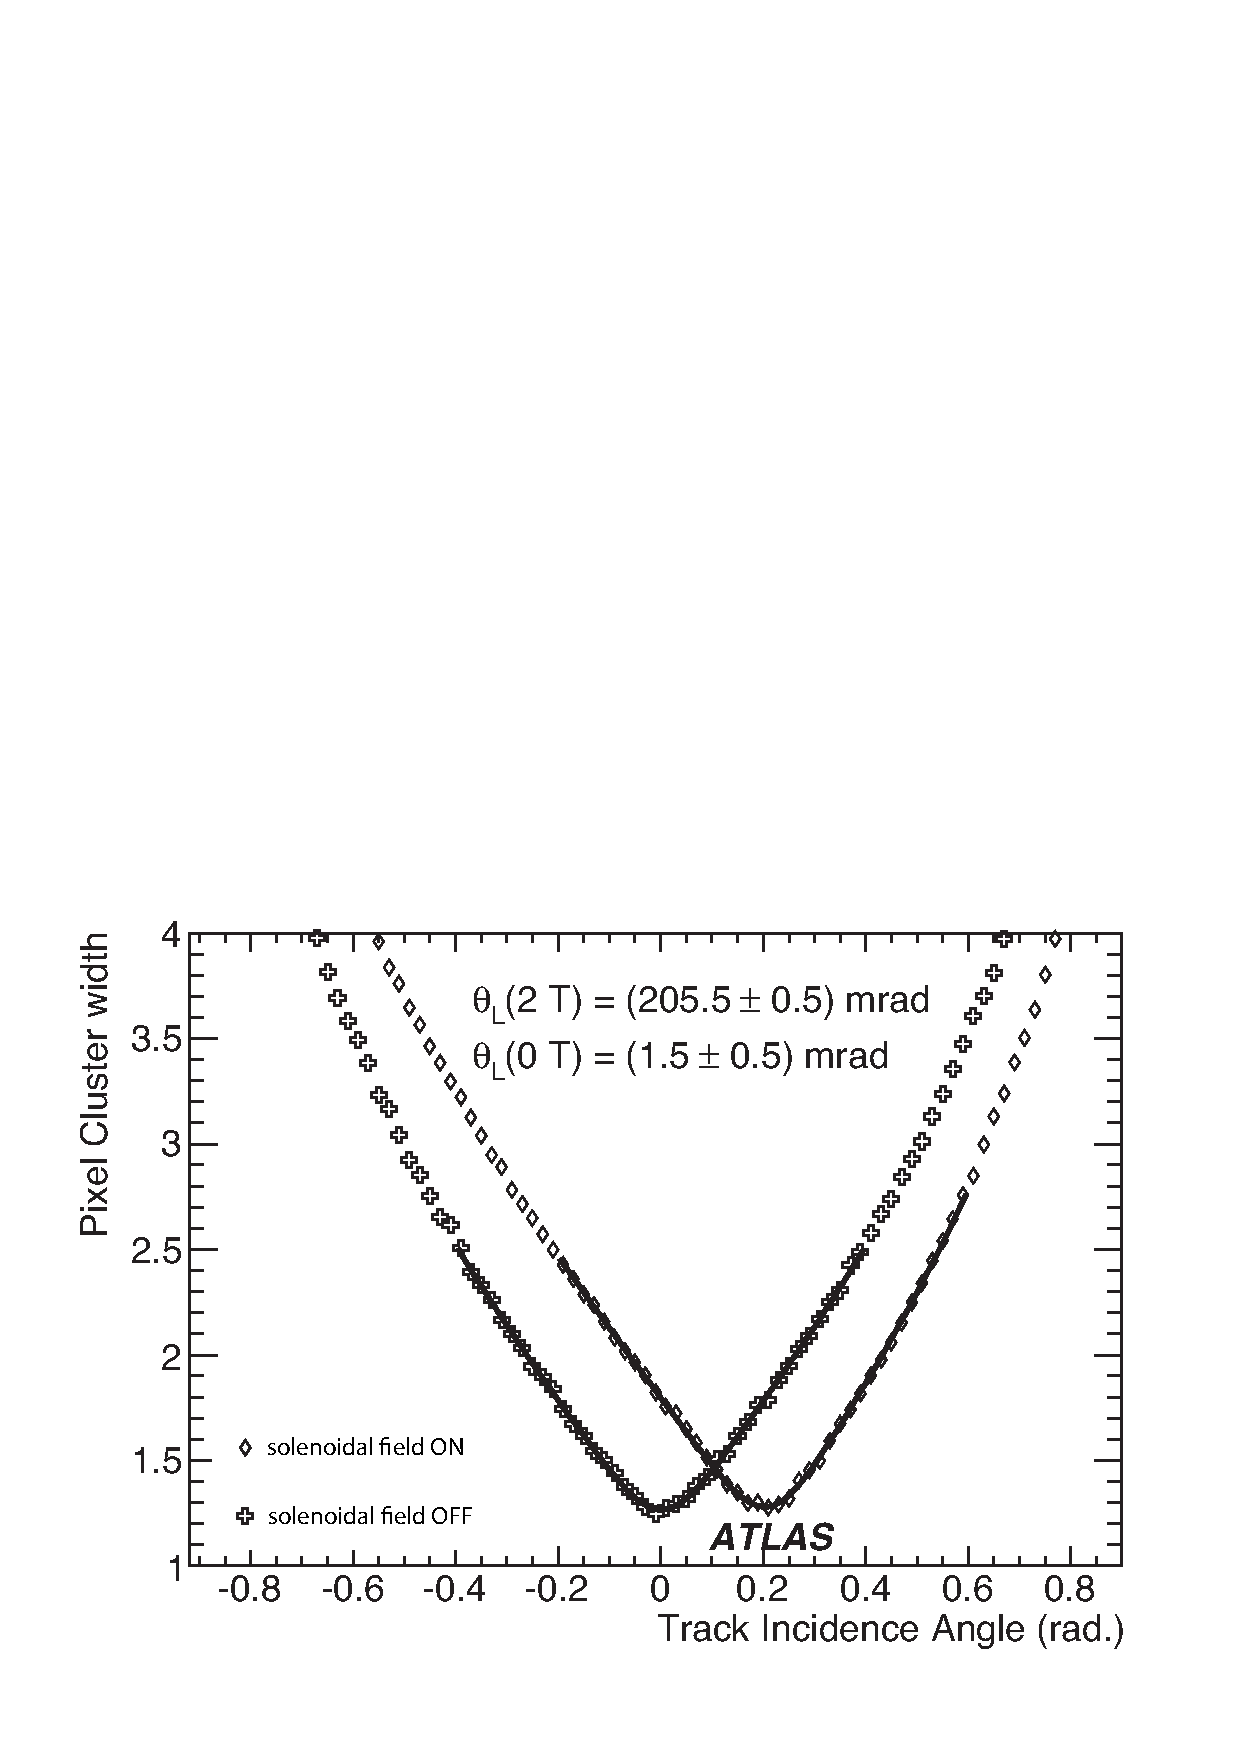
\includegraphics[width=0.5\textwidth,height=0.4\textwidth]{figures/SensorSimulation/LorentzConf3.pdf}
%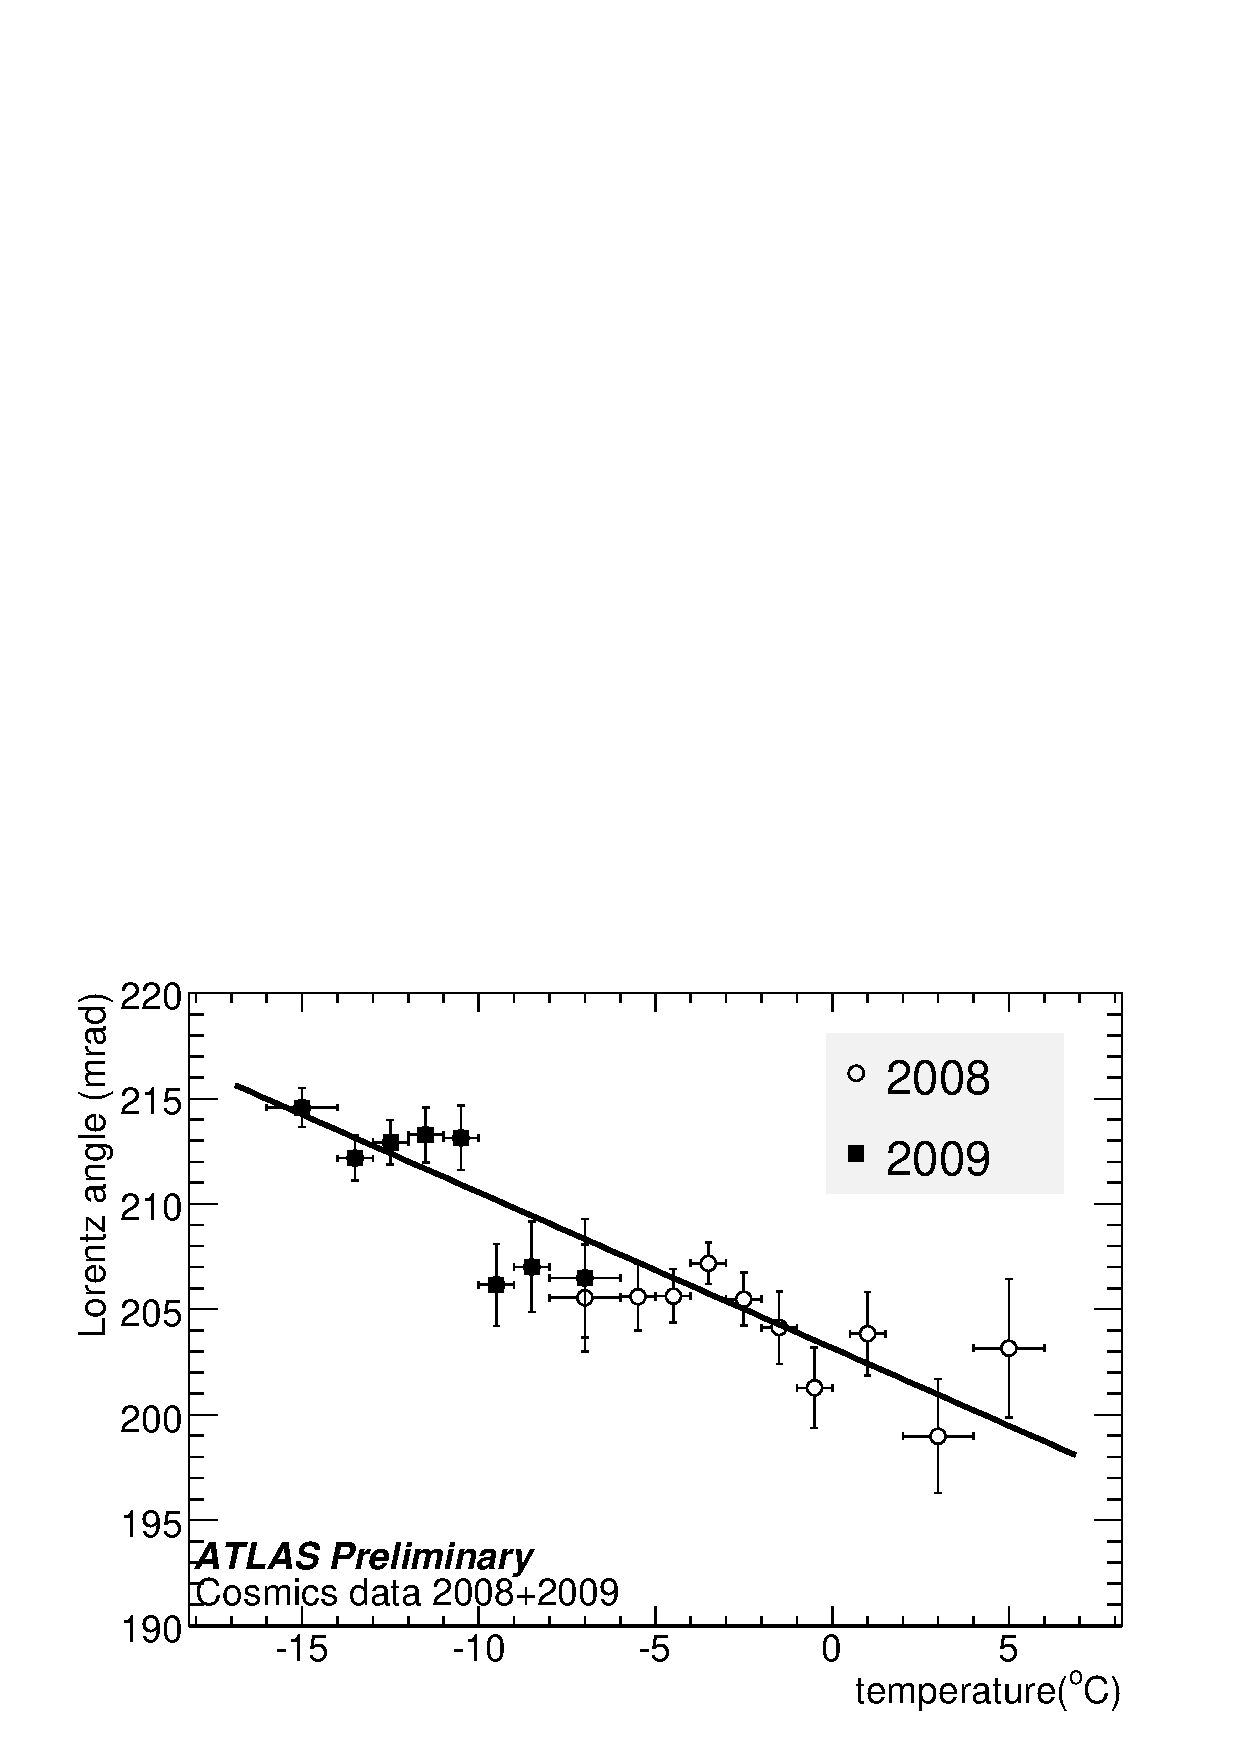
\includegraphics[width=0.5\textwidth,height=0.4\textwidth]{figures/SensorSimulation/LorentzVsTemp.pdf}
%\caption{Distribution of the cluster transverse size as a function of the incidence angle for cosmic muon events in which the magnetic field is turned off or set to 2 T, together with fits to analytic functions (left). Values of the Lorentz angle as a function of the temperature, together with a fit to a first-order polynomial (right).}
%\label{fig:cosmic1}
%\end{figure}
%\noindent
%The extracted values of the Lorentz angle are fitted as a function of the temperature to a first-order polynomial, yielding a slope
%\[
%\left(\frac{\partial\theta_L}{\partial T}\right)_{V_\mathrm{bias}} = (-0.74 \pm 0.03) \mbox{ mrad}\cdot\mbox{K}^{-1},
%\]
%in good agreement with the theoretical prediction of $-0.74 \mbox{ mrad}\cdot\mbox{K}^{-1}$~\cite{bib:jacoboni}.\\
%\newline
%Additional measurements of the Lorentz angle using cosmic muons were performed after the LHC Run I finished \cite{bib:cosmic2}. In this case, measurements were done separately on the different layers of the ATLAS pixel detector, showing differences between layers which can be interpreted as a result of the radiation damage after the Run I data-taking period. Figure~\ref{fig:cosmic2} shows the value of the Lorentz angle for B-Layer, Layer 1 and Layer 2, in comparison with the inclusive measurement from Ref.~\cite{bib:cosmic1}, discussed above. The value for the B-Layer is significantly larger than the ones from Layers 1 and 2, which are compatible with the 2009 results. Being the B-Layer closer to the beampipe, it is expected that this difference arises from a greater radiation dose, causing the Lorentz angle to increase.
%\begin{figure}[H]
%\centering
%\includegraphics[width=0.6\textwidth]{figures/SensorSimulation/cosmics.pdf}
%\caption{Comparison of the measurements in Refs.~\cite{bib:cosmic1} and~\cite{bib:cosmic2}, both using cosmic muons. The result in 2015 shows a larger value of the Lorentz angle for the B-Layer, which can be interpreted as a result of radiation damage.}
%\label{fig:cosmic2}
%\end{figure}
%\section{Mobility models}

%\subsubsection{Plans for Run 3 and the HL-LHC}
For future ATLAS physics in Run 3 and the HL-LHC, understanding radiation damage effects will be crucial. One possibility is to make the radiation damage digitizer a default component of the ATLAS simulation. Future challenges include deciding the exact fluences to use as simulation inputs, and also ensuring that the digitizer will run fast enough for bulk simulation production. 
 


\subsection{CMS}
\label{sec:CMS}
\subsubsection{CMS pixel detector}

 \paragraph{The CMS pixel detector and radiation damage effects}
 
The purpose of the CMS pixel detector sub-system is to precisely reconstruct charged-particle trajectories (tracks) from minimum ionizing particles (MIPs), that originate in proton collisions and pass through the silicon detector.
Such particles deposit charge by ionizing the silicon bulk: the deposited charge drifts through the sensor to an electrode, then the analogue signal recorded by the electrode is digitized, buffered and read out. 
To achieve a good resolution, each of the detector modules are designed to be thin, to be highly granular, and to have low occupancy.
In particular, the CMS pixel detector uses 285 $\micro m$ thick n in n sensors with 66560 pixels of cell size of $100\times 150 \micro m$.
Each sensor is mounted with modules containing readout chips (ROCs) of that are designed to withstand a high particle rate.
The full pixel system consists of a four-layer barrel detector (BPIX) and two endcaps in the forward regions, each comprising three disks (FPIX).
A full description of the CMS detector geometry and coordinate system can be found in~\cite{Chatrchyan:2008aa,tdr}.

Radiation damage can be caused by non-ionizing interactions from heavy particles and nuclei, these modify the sensor bulk and can alter the collected charge of MIPs~\cite{thesis,Aaboud:2019wgd}. 
The main modification to the sensor bulk comes from the displacement of a silicon atom out of its lattice site that results in a silicon interstitial state and a leftover vacancy. 
Both can migrate through the sensor and form clusters and point defects in the silicon lattice, that have energy levels in the middle of the forbidden gap. 
When activated and occupied, these states act as trapping sites and reduce the collected charge. 
%The trapping is due to the different time constants of the electron capture and emission processes. Traps are mostly unoccupied in the depletion region due to the lack of free charge carriers and can hold or trap parts of the signal charge for a time longer than the charge collection time and so reduce the signal height
They further act as recombination/generation centers and lead to an increase in the sensor leakage current.
This increase is proportional to the fluence received, $I_{\rm leak} \propto \Phi$, and translates to an increase in noise.
Finally they can also result in a change in the effective doping concentration, which is the difference of all donor-like states and all acceptor-like states.
Before irradiation, the depletion region grows from the back side of the sensor towards the pixel n$+$ implant.
After irradiation, the effective doping concentration decreases with increasing fluence until the sensor bulk undergoes space-charge sign inversion (or type inversion) from n-type to p-type.
The depletion region behavior is now like in p-material and grows from the n$+$ implant towards the back side of the sensor. 
Further irradiation leads to a gradual increase of the depletion voltage.
These effects are further complicated by the temperature history, since the thermal motion in the silicon lattice leads to an annealing current that causes new defects to be formed or existing defects to dissociate, cancelling the damage into the lattice.

In CMS, the modeling for radiation damage to the silicon sensors is performed with a standalone simulation (PIXELAV~\cite{pixelav,doublee}), that is independent from the full CMS Monte Carlo simulation framework (CMSSW). The results of the simulation are employed in the even reconstruction step of CMSSW. This is done by applying template corrections to the total deposited charge in simulation and further correcting the position of the reconstructed pixel hit. The next sections detail the PIXELAV simulation technique and the results of applying these corrections to CMS pixel data.

\paragraph{PIXELAV Simulation}

The detailed sensor simulation, PIXELAV, simulates the passage of a pion ($\pi$) through the sensor and incorporates the following elements:
\begin{itemize}
    \item An accurate model of charge deposition by primary hadronic tracks. This model uses the ``exact'' $\pi-e$ elastic cross sections of Bichsel~\cite{bischel}, that depend on the electron energy, to determine the $\pi$ mean free path.
    It takes into account the number of electron-hole pairs produced when the the scattered electrons or ``delta rays''  lose energy. 
    The total number of electron-hole pairs is chosen from a Poisson distribution where the mean number of pairs is determined assuming that it takes 3.68 eV to produce a pair. 
    The delta-rays are propagated until they lose all energy or they leave the sensor.
    \item A realistic electric field profile resulting from the simultaneous solution of Poisson’s Equation, carrier continuity equations, and various charge transport models. This full three dimensional electric field map is generated with the  TCAD package~\cite{tcad}.
    It predicts a non-uniform spatial distribution of space-charge density for computing charge propagation inside the sensor bulk.
    \item A model of charge transport inside the sensor. 
    The electrons and holes produced by the primary hadron drift to the sensor implants under the influence of the internal electric field and the external magnetic field.
    They drift with a carrier-dependent mobility ($\mu$) that depends on the electric field (E) and temperature.
    The model of the charge transport includes the charge carrier mobility and Hall Effect and 3-D diffusion.
    \item A simulation of charge trapping and the signal induced from the trapped charge after radiation exposure. 
    When charge carriers are trapped they  are captured for periods of time that are long as compared with the integrating time of the pre-amplifiers and are not detected with full efficiency.
    This trapping time is incorporated in the simulation by halting the propagation of that charge carrier according to the effective trapping times measured in~\cite{kram}.
    After all charge carriers have reached the boundary of the detector or have been trapped, the program counts the number of electrons that have been collected by each n$+$ implant.
    Then it calculates the additional charge induced on each pixel by trapped electrons and holes by approximating the detector as a parallel plate capacitor with a rectangular segment anode.
\end{itemize}

For each event, the simulation outputs the coordinates of the pion entry and direction, the generated number of electron-hole pairs, and two sets of signals for a pixel array.
The first set includes only collected electrons and the second set includes collected electrons and induced signals from trapped charge.
The final step consists in a simplified simulation of the electronics and readout system.
First, a random noise is added to each pixel signal.
Then, a function that simulates the analog response of the ROC is applied to the total signal.

The simulation was originally written to interpret beam test data from several un-irradiated and irradiated sensors. 
In CMS, the simulation is used to produce cluster projection shapes, also called ``templates'', across measured cluster projections. 
These templates are produced for different incident track angles ($\cot \alpha, \cot \beta$) and positions. 
They take into account the sensor geometry and are produced under certain conditions of fluence, temperature, bias voltage and magnetic fields.
A single cluster template is created by repeatedly simulating the particle traversal for a certain incidence angle and position within a pixel using the pixelav software.
CMS has developed techniques to tune the Pixelav trapping parameters from collision data through measurements of the charge collection vs depth.
The templates produced from the tuned PIXELAV simulation are used to find the best fit and hence an estimate of the hit position in both x and y. 
Furthermore, they are used to re-weight the digitized cluster charge profile as a function of the production depth.
These applications are detailed in the next section.


\paragraph{Corrections in the pixel hit reconstruction}
The main usage of the PIXELAV templates in CMS is through the template-based reconstruction algorithm. This algorithm aims to get a better estimate of the pixel hit position by accounting for the charge sharing functions of the detector and how they are modified during large portions of its useful life. This is possible through the use of all the projected pixel information.

The technique is based on fitting the pixel cluster X and Y projections to the pre-determined cluster shapes or templates produced with PIXELAV. 
Given a track with angles $\alpha$ and $\beta$ incident to the pixel module, the pre-determined cluster template is compared to the actual cluster produced by the track in question. 
A $\chi^2$ minimization is performed with hit $X$ and $Y$ positions as floating variables.
The hit position is given by the $X$ and $Y$ coordinates which minimize the $\chi^2$ comparison.

The cluster template technique was originally developed to optimally estimate pixel hit position after radiation damage, but it was found that it performs better than standard CMS pixel hit reconstruction~\cite{standard} even before irradiation. 
The technique requires knowledge of the track direction, so it is used in the second pass of pixel hit reconstruction, when track incidence angles on detector modules are known. 
In the first pass of the reconstruction the standard technique is used.
Results of this method are detailed in ~\cite{pixelhit}.

\paragraph{Pixel cluster charge reweighting}
The pixel charge profile is defined as the normalised average pixel charge as a function of the production depth.
For a non irradiated, fully depleted detector, the pixel charge profile is expected to be flat as the detector is fully efficient and all the charge is collected. 
While, for an irradiated detector charge collection losses are expected due to the trapping of carriers. 
The losses are larger for the charges released further from the readout plane.
This behavior is shown in Fig.~\ref{fig:charge} for different data 2018 taking scenarios.
During the 2017 Extended Year Technical Stop, 
the Barrel Pixel detector was held at the temperature above 10\textdegree{}C for 53 days. 
The beneficial effect of the annealing during this period is clearly visible in the flattening of the pixel charge profile.
At the beginning of 2018 data taking, the charge collection was additionally increased in Layer 1 by raising the bias voltage from 350 V to 400 V.

\begin{figure}[htp]
\centering
\includegraphics[width=0.40\textwidth]{figures/SensorSimulation/norm55_v1.png}
\caption{ Average pixel charge as a function of production depth. 
The charge distribution is shown the Layer 1 of the CMS Barrel Pixel detector at the end of 2017 (HV = 350 V), at the beginning of 2018 data taking (HV = 350 and 400 V) and after 30.0 fb$^-1$ of data collected in 2018. 
The selection includes tracks with $p_T > 3$~GeV, pixel cluster charge $ <~1000~ke^{-}$, cluster size in $y < 4$ and hit position residuals $< 100 \mu m$.
}
\label{fig:charge}
\end{figure}

The Cluster Charge Re-Weighting (CCR) algorithm attempts to describe this behavior.
This algorithm modifies the charges in a cluster arising from a single simulated hit such that a better description of the sensor response is obtained, while maintaining the randomized nature of the signal creation process. 
The method of CCR sets in at the end of the first part of the digitization process and is applied to clusters of pixel charges resulting from a single primary particle. 
Therefore, in CMSSW, the CCR is implemented before the charges in the pixels are summed and thresholds are applied.

To apply the CCR to a simulated cluster, the incidence angle and position of the corresponding primary particle and the module ID are used to find the most suitable cluster templates from the set of PIXELAV templates.
These are generated for various incidence angles and positions, as well as for different levels of irradiation.
The templates are read from a database, and an interpolation is performed between the simulated particle parameters. 
The original$_{x,y}$ induced charge of a pixel in the cluster is then scaled with the quotient $w$ of the template pixel charges at the same position inside the cluster for an irradiated ($t^{\rm irr}$) and an un-irradiated sensor ($t^{\rm unirr}$). 
A matrix of $13\times21$ pixels is defined, which covers the full cluster and has the particle hit position in its center. 
For any pixel, specified by its pixel coordinate $(x,y)$ with respect to the lower left pixel of this matrix, the re-weighted charge $signal_{x,y}$ is determined as
\begin{equation}
    \text{signal}_{x,y} = \frac{t^{\rm irr}_{x,y}}{t^{\rm unirr}_{x,y}} \times \text{original}_{x,y}
\end{equation}

For pixel charges of the templates below a defined threshold, no weights are computed, and instead the pixel charge is computed using the weight of the closest pixel with a weight.

One way to verify the effect of the CCR is to extract the collected charge as a function of the charge carrier creation depth from very long clusters. 
For unirradiated sensors, this profile is flat, and it is tilted for strongly irradiated sensors, as shown in the following graph. 
The CCR can reproduce this effect. This is shown in a preliminary distribution of the average charge profile in Fig.~\ref{fig:ccr}.

\begin{figure}[htp]
\centering
\includegraphics[width=0.40\textwidth]{figures/SensorSimulation/chargeProfileAll.png}
\caption{ Average pixel charge as a function of production depth for the Layer 1 of the CMS Pixel Barrel detector for one particular run at the end of 2017. 
The profile of the data collected in the Run 304292 (green) shows the losses expected due to the trapping of carriers as a function of depth. 
The charge simulation without the CCR algorithm is flat and shown in red.
After applying the CCR algorithm a more accurate description of the simulated charge profile can be seen in blue.
}
\label{fig:ccr}
\end{figure}

The PIXELAV simulation was originally developed to interpret beam test results and is now a key part of the digitization and reconstruction algorithms in the CMS simulation framework.
It was developed to model pixel sensor physics as accurately as possible but its speed is not optimized to be included as part of the main CMS simulation framework.
Therefore, its usage is limited to estimate the radiation damage effects in an standalone mode.
Specifically it provides a more accurate estimate of the pixel hit position in the event reconstruction and is used to implement corrections to the simulated pixel cluster charge profiles.
The latter is performed through a re-weighting algorithm that include more realistic modelling and irradiation effects. 
The simulation and the reconstruction are currently being synchronized by using templated cluster shapes generated from the same models.
Preliminary cluster profiles measured in data and simulation show encouraging and promising results that reflect a more accurate estimate of the radiation damage effects.


\subsubsection{CMS strip tracker}
The CMS tracker~\cite{CMS:1998aa,CMS:2000eqx} is the largest silicon tracker in the world.
It consists of 10 layers of silicon in the barrel 3 inner and 9 endcap disks. 
The detector contains 15,148 modules with more 9.3 million silicon strips covering a total active area of silicon of 198 m$^2$.
Strip sensor thicknesses are 320$\micro$m up to a radius of 600 mm, and 500 $\micro$m at larger radii.
The charge on each microstrip is read out and amplified by an Analogue Pipeline Voltage (APV25) chip.

The GEANT4 package that describes the energy loss in the CMS tracker based on the interactions between the incoming particles and the bulk of silicon sensor is not sufficient to simulate the signal collected in the real detector.
For radiation damage in the CMS strip tracker, an experiment-specific simulation of the signal and noise is required. This has been implemented within the CMS Software (CMSSW) framework.

For a given silicon strip module whose geometry is known, the simulation \cite{Ranieri:1103455} starts from G4 hits providing information about the direction of the incoming particle, a hit position in the local frame and the total energy loss.
The first step consists in dividing the trajectory of the incoming particle and randomizing the energy loss in each sub-paths following a Landau distribution.
The second step simulates the charge carrier drift including the thermal diffusion of the charge carriers.
The underlying hypotheses are that the  E-field is normal to the sensor plane and that there is no charge collection inefficiency.
The next step emulates the effect of the inter-strip capacitance which induces charges in strips  neighbors of the one collecting the charge carriers.
This is performed through a parametrisation of the cross-talk effect
assuming that for a given charge $Q$ collected on a strip $i$, the signal observed on that strip will be $x_0\times Q$, the two closest strips $i\pm 1$ will measure a charge $x_1 \times Q$ and the second ones ($i\pm 2$) a charge $x_2 \times Q$.
The parameters are constrained by the relationship $x_0+2x_1+2x_2 = 1$.
The parametrization depends on the detector geometry and the readout mode of the APV25 (peak or deconvolution).
To simulate the front-end electronics, a parametrization of the pulse shape is provided for both readout modes.
It is assumed that the detectors are synchronized and that the signal of ultra-relativistic particles are sampled at their maxima.
Consequently, the signal collected for low $\beta$ particles, loopers, as well as out-of-time pile effect induced by the electronic response are properly simulated.
The above described simulation chain produces simulated hits ({\bf SimHits}).

The next goal consists in simulating the digital data acquired by the back-end electronics (front-end driver, or FED), called the {\bf digis}.
Contributions from all particles, including in-time and out-of-time pileup, are summed. The list of bad components is extracted from an offline database and is used to suppress signal for the corresponding channels.
In order to describe the noise, it is required to randomize the summed signal according to the knowledge of the noise in each channel.
This information is also provided by the offline database. 
To simulate the optical chain response where gains vary between links, values of 
gains per APV stored in the database are used.
The last elements in the readout chain are the FED where the digitization, a zero suppression and a cluster algorithm are performed.
The signal processing in the FED is emulated in the CMSSW framework leading to 8 bits digis as provided during data-taking.


 
To be as realistic as possible, it is better to use quantities extracted from measurements to feed the offline database.% with payloads latter used for simulation. 
During run II, the bad component list, the noise, the gains, the cross-talk parameters and the APV signal shape have been measured.
After some basic treatments, those measurements have been used to either feed the database or to update parameters stored in configuration files.
The noise is measured simulateously with the pedestals during calibration runs where no collision occur.
The APV signal shape is measured with charge injection 
%and the us of delay in the PLL providing an e
to estimate of the electronic response.
However to simulate the observed signal, it has been required to convolute it with a physical signal simulated with external tools.
The gains of the optical chains are measured thanks to reference signal, called tickmark, in devoted runs.
The cross-talk parameters have been measured in cosmic runs without magnetic field to avoid lorentz deflection and in virgin raw data-taking mode where no zero supression is performed, in order to avoid threshold effect.

All those quantities have evolved with time and needed an update.
In order to validate the simulation, data/MC comparisons have been performed focussing on the most relevant quantities, mainly the cluster charge and width.
The cluster charge is in general, very well reproduced thanks to the gains.
More recently, for the Run II ultra-legacy campaign in CMS, a simulation of the preamplifier has been introduced.
It simulates the non linear response observed in case of high flux operation.
This effect which depends on the electronics configuration, was unfortunately amplified beginning of run II due a bad configuration and leading to dynamic inefficiency impacting the tracking efficiency in data-taking up to summer 2016.
This effect is now propagated into the simulation and improves the simulation especially  the description of the low charge contributions.
The APV signal has mainly changed due to a reparametrization of the electronics.
The update impacts off-time signals description.
The noise decreased with change of the operating temperature but increased with irradiation.
An update of the noise helps to better describe the drop of signal-over-noise ratio which was measured in the data and reported in the left plot of the figure \ref{fig:SiStripPlots}.
It also has an impact on off-track clusters and the low charge description of the on-track clusters. 
The cross-talk is related to the inter-strip capacitance which is affected by surface damages and depends on bias voltage.
A comparison of the parameters for the barrel detectors are reported in right plot of the figure \ref{fig:SiStripPlots}.
The cluster width description has significantly been improved  thanks to the update of the cross-talk parameters.
While descrepancies still remain, they do weakly impact downstream quantities.
The optical link gain decreased with time due to a loss of efficiency in the AOH and a loss of transparency in the optical fibers. 
The update of the gains help to better describe the fraction of channels having signal saturating the 8-bit ADC.


Measurement of the hit efficiency as function of the pileup shows a linear dependancy.
The source of ineffiency has been indenfied has originating from heavy ionizing particles, i.e., inelatic nuclear interaction within the active volume.
The ineffiency does not exceed 2\% even at high pileup and for innermost layers.
A simple approach to simulate ineffiency exists in the simulation but has not been activated in the recent campaign.

To conclude, the tracker simulation have been updated using the best knowledge we have on the detector throught updates of the database payloads and parameters.
Moreover a simulation of the preamplifier have been developed mainly to better describe the data in the first periods  of 2016 where the silicon strip tracker suffered from dynamic inefficiencies.
Beyond similar updates that will need to be performed during run III, two kinds of improvements could be foreseen.
The inclusion of the HIP-induced hit inefficiency could be used in production.
Moreover, as the detector will suffer even more from irradation, a drop of charge collection efficiency is expected to be observable in the innermost layer.
After a dedicated measurement,  this effect could be  injected into the simulation to even better describe the signal-over-noise ratio.

In general, the validation of the simulation shows that the track reconstruction and downstream algorithms are quite robust and do not require an very fine level of accuracy in the simulation.


\begin{figure}
\center
\label{fig:SiStripPlots}
\caption{On the left, evolution of the signal-over-noise ratio for modules belonging to different partition. Higher ratio correspond to the thick (500 $\mu m$) sensors.
On the right, cross-talk parameters for the 4  barrel silicon strip sensor geometry measured in run I and run II. 
}
\includegraphics[width=0.48\textwidth]{figures/SensorSimulation/StoNTrend_graph.pdf}
\includegraphics[width=0.48\textwidth]{figures/SensorSimulation/Xtalk2018.pdf}
\end{figure}


\subsection{LHCb}
\label{sec:LHCb}
High-quality simulation is of major importance for LHCb experiment. The overall strategy is identical to
each sub-detector that exploits silicon-based devices and may differ in some details related mainly to the
emulation of the readout electronics. The full processing chain leading to the production of simulated
samples is divided into three independent stages:
– generation of proton-proton interaction with a particular final state particles and their propagation
through the detector (simulation phase),
– simulation of the detector response (digitisation phase),
– detector output data decoding, track finding and fitting (reconstruction phase)
In the first stage, that is also the most time consuming one, the full truth information (a particle
4-momenta and its identification) is used by the LHCb Gauss application \cite{lhcb1} to simulate the effects of
the passage of particles through detector material. Gauss is interfaced with Geant4 \cite{lhcb3} package that is
dedicated to simulating with great precision effects such as energy loss or multiple scattering. The results
are then stored in a specialised class called MCHit. The next stage, performed by the LHCb application
Boole \cite{lhcb2}, uses the MCHit objects to perform the detector response simulation (see Section 2). Also,
the output of Boole is formatted in an identical way it is sent out to processing in the trigger farm by the
respective detectors. Finally, the LHCb Brunel application \cite{lhcb4} is used to produce tracks and vertices that
are stored in DST files. Brunel is data-type agnostic, i.e., both simulated and collision data are processed
in the same way. Also the simulated DST files can be further processed in an identical manner as real
data are.

The MCHit objects that are produced by Gauss application and contain such data as sensitive material
entry and exit points and energy loss are subsequently used to simulate detector hits. Using the deposited
energy value for each particle, the corresponding number of electron-hole pairs are calculated. This
generated charge is then distributed along a particle’s path within the silicon. The deposition process
progresses in steps (where the number of steps is a tunable parameter) and has three components: the
constant core ionisation, random ionisation and high energy $\delta$-ray emission. The relative contribution
of these three components is tunable, although, the high energy electron production is simulated in "a
posteriori mode". The energy of emitted $\delta$-rays is recovered by comparing the total generated charge and
distributed one - if the difference is larger than a given cutoff value the emission process is simulated at a
randomly chosen point on the particle’s path within active material. Finally, the total distributed charge
is normalised to the total generated charge for the consistency.
The distributed charges are then propagated through the sensitive material using a simple projection method that is also the fastest one. At each point, a random lateral diffusion is estimated by
sampling a Gaussian distribution and then the charges are placed at the surface of the sensor. At this
point, radiation damage effects are taken into account, if necessary, changing appropriately the collected
charge distribution. In this pragmatic approach, a simple linear electric field is assumed, and no transient
currents are simulated at the sensor collecting electrodes. Using local information on sensor segmentation topology from a detector model description, a list of channels with collected charges is created.

The list is next passed to the readout emulation code that adds electronic noise, introduces capacitive
couplings between channels, perform digitisation and finally applies activation cuts (zero suppression)
and performs clusterisation (hit reconstruction). The last step is the cluster data encoding into the format
that is identical with the transport protocol of respective detectors (also called RawBank) that is the input
data for the LHCb Brunel application for track reconstruction. In order to reproduce the clusterisation
and encoding exactly the emulation and calibration software were partially ported into the simulation
platform \cite{lhcb6}.


The results of the simulation process can be broadly divided into two categories: low level including
Landau distribution of deposited energy and its dependency on the local position on a sensor, hit rates,
occupancies etc., and high-level such track multiplicity, primary and secondary vertices, single hit reso-
lution, vertex resolution, geometrical impact parameter resolution etc.

\begin{figure}[]
    \centering
    \includegraphics[width=0.45\textwidth]{figures/SensorSimulation/adc_data.pdf}
    \includegraphics[width=0.45\textwidth]{figures/SensorSimulation/adc_mc.pdf}
    \caption{
Energy distribution, measured in arbitrary ADC counts, fitted with a model representing Landau convoluted
with a Gaussian for a selected VELO sensor. Left hand-side plot is obtained using collision data whilst the right-
side hand one presents simulated data. Plots are not normalised.
}
    \label{fig:adc}
\end{figure}

The latter set of variables need full track reconstruction to be performed. Some of these observ-
ables are of the out-most importance and are very often compared to the corresponding ones obtained for

the data. Specifically, the primary vertex resolution (life-time measurements), impact parameter resolu-
tion (selection algorithms), spatial resolution (track fitting) and Landau distributions (hit reconstruction

and their association to tracks and radiation damage studies) are being carefully monitored. Below we
present selected results: the Landau curves and spatial single hit resolution.

\begin{figure}[]
    \centering
    \includegraphics[width=0.45\textwidth]{figures/SensorSimulation/reso.pdf}
    \includegraphics[width=0.45\textwidth]{figures/SensorSimulation/reso_projectedangle.pdf}
    \caption{
Single hit spatial resolution measured for the LHCb VELO detector. Right-hand side plot shows the
resolution as a function of the sensor pitch for two different track angles and compared to the binary one; the
right-hand side plot shows the resolution as a function of track angle for different pitch regions.
    }
    \label{fig:resolution}
\end{figure}

The silicon simulation software is an essential part of the detector performance studies (including ra-
diation damage effects) and physics analyses performed by LHCb collaboration. The quality of the
simulated samples is continuously improved and cross-checked against the collision data. The constant
maintenance and improvements of the simulation code, often using the feedback from measurements, is
crucial.


\subsection{ALICE}
\label{sec:ALICE}

After the second LHC Long Shutdown (LS2), the luminosity with lead beams will gradually increase to an interaction rate of 50 kHz, %a rate that the current ALICE experiment is unable to deal with. 
leading to a data rate that the current ALICE electronics and detectors cannot process. The upgrade of the experiment is mainly focused on increasing the readout rate capability to record the full 50 kHz of Pb-Pb interactions (and to collect reference data for heavy-ion measurements up to few 100 kHz for high luminosity pp and p-Pb collisions). In addition, the detector capabilities will be enhanced to perform precision measurements of the following topics in heavy-ion collisions: study of heavy quark thermalisation, measurement of low-mass dileptons and thermal photons, measurements of gamma-jets with particle identification and search for exotic heavy nuclear states. A detailed description of the general ALICE upgrade program and the physics goals can be found in the ALICE Upgrade LOI~\cite{upgrade}. In the extended running scenario for {\sc run} 3 and 4, summarised in Table ~\ref{scenario} and even more ambitious than the plan reported in the LOI, the ALICE experiment intends to accumulate 13\,nb$^{-1}$ of Pb--Pb events at $\sqrt{s_{NN}}$ = 5.5 TeV (10\,nb$^{-1}$ at full magnetic field and 3\,nb$^{-1}$ at reduced field), 1 pb$^{-1}$ of p--Pb and 6 pb$^{-1}$ of pp reference data at the equivalent Pb nucleon energy, and 250 pb$^{-1}$ of pp collisions at $\sqrt{s}$ = 14 TeV. The last row in Table \ref{scenario} represents the expected total number of charged particles per unit of pseudorapidity integrated for {\sc run} 3 and {\sc run} 4. 


\begin{table}[ht!]
\begin{minipage}{\textwidth}
\begin{center}
\begin{tabular}{l c c c}
\toprule
								& pp 					& p--Pb 	 			& Pb--Pb	\\
								& 14 TeV				& 5.5 TeV/$NN$		& 5.5 TeV/$NN$ \\
\midrule
$\int \mathcal{L} (\rm{nb}^{-1})$	 		& 2.5 10$^{5}$			& 1000				& 13		\\
$L_{peak} (\rm{cm}^{-2}\rm{s}^{-1})$		& 6.0 10$^{30}$		& 1.0 10$^{29}$		& 6.25 10$^{27}$	\\
$\sigma_{\rm t}$ (mb)				& 80					& 2000				& 8000 	\\
Peak rate (s$^{-1}$)					& 4.2 10$^5$			& 2.0 10$^5$			& 5 10$^4$	\\
Events							& 2 10$^{13}$			& 2.0 10$^{12}$		& 10.4 10$^{10}$	\\
\dndeta							& 6.46				& 18.4				& 492.5		\\
\midrule
peak rate of tracks $N_{ch}/\eta  \, (s^{-1})$   	& 2.7 $10^6$  		& 3.7 $10^6$ 			& 25 $10^6$ \\
total Nr. of tracks $N_{\rm{tot}}/\eta$			& 129.2 10$^{12}$	& 36.8 10$^{12}$		& 51.2 10$^{12}$	\\  
\midrule	
\end{tabular}
\end{center}
\caption{Extended running scenario for the ALICE operation after LS2. $\int{ \mathcal{L}}$ and $L_{peak}$ stand for integrated and peak luminosity respectively, $\sigma_{\rm t}$ for inelastic cross section and $\eta$ for pseudorapidity. }
\label{scenario}
\end{minipage}
\end{table}

%Since the radiation load is strongly correlated to the total number of produced particles one can infer that the contribution of Pb--Pb runs is dominant. The planned pp and p--Pb collisions represent together only 7.9$\%$ of the Pb--Pb Total Ionising Dose (TID) and high-energy hadrons fluence numbers (precisely 4.3$\%$ and 3.6$\%$, respectively). The fluence rate is proportional to the product of interaction rate and particle multiplicity and is therefore highest for Pb--Pb collisions. In conclusion, the Pb--Pb operation represents the most hostile environment in terms of total fluence ($51\times10^{12}$ charged particles per unit of rapidity) and fluence rate (25\,MHz of charged particles per unit of rapidity).\\
\noindent Since the radiation load is directly correlated to the total number of produced particles, the planned pp collisions represent the 59$\%$ of the Total Ionising Dose (TID) and high-energy hadrons fluence numbers, while p--Pb and Pb--Pb collisions account for 17$\%$ and 24$\%$, respectively. The fluence rate is proportional to the product of interaction rate and particle multiplicity and is therefore highest for Pb--Pb collisions. In conclusion, 
due to the longer running time the largest contribution to the total fluence is given by pp operation ($129.2\times10^{12}$ charged particles per unit of rapidity), while Pb--Pb operation represents the most hostile environment in terms of fluence rate (25\,MHz of charged particles per unit of rapidity).\\


\subsubsection{Radiation load simulations}

The radiation load for the upgraded program has been estimated with dedicated simulations to derive the radiation specifications for detector and electronics prototypes. More details can be found here~\cite{RadNote}.\\
During {\sc run} 1, after the beam ramp-up intensity in 2011, a degradation of the vacuum upstream the ALICE detector was observed, producing a large background in the experiment. Pressure bumps starting during the beam injection and reaching about 4--5 $\times 10^{-8}$ mbar, and lasting a large fraction of the fill duration were observed, affecting the experiment running, since all gaseous detectors could not be ramped up at nominal setting due to very large rate resulting in high--voltage trips. 
The sources of this large background were mainly dynamical effects as ion, electron and photon-induced gas desorption and electron cloud formation. A large pressure increase has also been observed inside the injection beam stopper (TDI), ascribed to impedance heating induced by circulating beams.
This machine--induced background was substantially cured during the first Long Shutdown (LS1); however, since it might have a non negligible impact on the radiation load, its contribution was simulated and accounted for in the final calculations.\\
The radiation simulations are performed within the AliRoot \cite{AliRoot} framework, which provides a detailed geometry and material description of all detector layers, support structures and beamline elements inside the ALICE experimental area. Electric and magnetic field maps are processed as well. The simulated geometry assumes still the present Inner Tracking System (ITS) detector with detailed implementation of services and support structures. Since the upgraded ITS will use ultra light structures, optimized for minimum material budget, the simulations for the present ITS are conservative in terms of radiation effects.\\
The particle transport is performed with FLUKA \cite{fluka}. The transport cuts for the particle species are adjusted region by region according to their importance in order to optimize the computing time. The lowest cuts are used in the central barrel detectors, while in the outer regions these cuts are raised considerably in order to save CPU time. The lowest kinetic energy cutoff for photon, electron, neutral and charged hadron and muon transport is set to 1 keV and down to thermal energies of 293 K for neutron. The threshold for electron and muon delta-ray production is 30 keV, as well as for electron and muon bremsstrahlung and for electron pair production by muons.\\
The calculations of the radiation load from Interaction Point (IP) collisions are based on 50000 minimum bias pp events at a centre-of-mass energy of 5.5 TeV simulated using the PYTHIA \cite{pythia} event generator (Perugia-2011 tune);  results for p--Pb and Pb--Pb collisions, as well as for pp collisions at a centre-of-mass energy of 14 TeV, were derived by scaling the pp values by the average charged-particle multiplicity density reported in Table \ref{scenario}, under the assumption that the shape of the \dndeta \ distribution does not differ significantly for the different colliding systems. The charged-particle multiplicity densities at midrapidity have been obtained by scaling the ALICE measured multiplicities \cite{pp, pPb, PbPb, PbPbbis}. A scaling factor of $s^{0.15}_{NN}$ ($s^{0.11}_{NN}$) has been applied to Pb--Pb (p--Pb and pp) to obtain the values for the centre-of-mass energy of $\sqrt{s_{NN}}$ = 5.5 TeV.\\
The hadron fluence, quoted in 1-MeV neutron equivalents (neq) and quantifying the Non--Ionising Energy Loss (NIEL), and the TID are the numbers that determine the long term radiation damage of sensors and electronics.
The rate of hadrons with a kinetic energy $>$ 20 MeV determines the rate of stochastic failures, like single event upsets in the microelectronics circuitry. The fluence of all the charged particles is not directly linked to radiation-induced effects; nevertheless it determines the detector occupancy and influences track reconstruction and particle identification and was therefore calculated along with the above mentioned quantities.
The FLUKA USRBIN function, that allows the distribution of one or several quantities of interest to be scored in a regular spatial structure independent from the geometry, is used in the calculations. All results were obtained by superimposing a $r-z$ cylindrical mesh, with the cylinder axis parallel to the $z$-axis, on top of the ALICE geometry; the scored quantities are averaged along the azimuthal angle $\varphi$. Results from the USRBIN function are normalised per unit volume and per unit primary weight.\\
Different meshes were defined to score the relevant quantities with the appropriate granularity. The bin size ranges from 1 mm $\times$ 5 mm for the innermost layers of the silicon detectors to 1 cm $\times$ 2.5 cm for the outermost ALICE detectors.

\begin{figure}[t]
\centering
\includegraphics[width=0.95\textwidth]{figures/SensorSimulation/dose2.png}	
\caption{Map of the Total Ionizing Dose (in krad) for an integrated Pb--Pb luminosity of 10\,nb$^{-1}$ in the ALICE central barrel. The schematic of the ALICE geometry in $r-z$ coordinates is superimposed.}
\label{dose} 
\end{figure}

\begin{figure}[H]
\centering
\includegraphics[width=0.95\textwidth]{figures/SensorSimulation/nequ2.png}	
\caption{Map of the NIEL weighted 1-MeV-neq fluence (in cm$^{-2}$) for an integrated Pb--Pb luminosity of 10\,nb$^{-1}$ in the ALICE central barrel. The schematic of the ALICE geometry in $r-z$ coordinates is superimposed.}
\label{neq} 
\end{figure}

\begin{figure}[!ht]
\begin{center}
\includegraphics[width=0.95\textwidth]{figures/SensorSimulation/hadron2.png}	
\end{center}
\caption{Map of the fluence rate of hadrons with kinetic energy in excess of 20\,MeV for a Pb--Pb collision rate of 50 kHz, expressed in kHz/cm$^{2}$. The schematic of the ALICE geometry in $r-z$ coordinates is superimposed.}
\label{had} 
\end{figure}

\begin{figure}[H]
\begin{center}
\includegraphics[width=0.9\textwidth]{figures/SensorSimulation/charged2.png}	
\end{center}
\caption{Map of the charged-particle fluence rate for a Pb--Pb collision rate of 50\,kHz, expressed in kHz/cm$^{-2}$. The schematic of the ALICE geometry in $r-z$ coordinates is superimposed.}
\label{ch} 
\end{figure}


\noindent Maps of the TID and the NIEL, quoted in 1-MeV-neq fluence, are shown in Figures \ref{dose} and \ref{neq} for genuine IP collisions and an integrated Pb--Pb luminosity of 10 nb$^{-1}$. The fluence rate of hadrons with a kinetic energy greater than 20 MeV is shown in Figure \ref{had}, while Figure \ref{ch} shows the fluence rate of all charged particles; both maps are produced assuming 50 kHz of Pb--Pb collision rate.\\
At positions with $-$100 $< z <$ 350 cm, the radiation numbers are dominated by primary tracks originating from the interaction point. At $z <$ $-$100 cm the front absorber of the Muon Spectrometer is stopping hadrons that are pointing towards the muon system, which leads to a decrease of the TID but an increase of the hadron fluence due to the lateral escape of neutrons. The innermost ALICE detectors are exposed to a TID close to 0.1\,Mrad (1 rad = 0.01 Gy) and a 1-MeV-neq hadron fluence up to 10$^{12}$  $\rm{cm}^{-2}$. The flux density of high-energy hadrons for these detectors is expected to reach 0.7 MHz/$\rm{cm}^{2}$. The ALICE Time Projection Chamber (TPC) electronics located at the inner radius of the service support wheel has to stand a dose of up to 0.25\,krad and 1.8\,kHz of high-energy hadrons.


\paragraph{Contribution of beam-gas background}

The machine-induced background is mainly ascribed to inelastic interactions of beam protons with residual gas molecules in the so-called Long Straight Section (LSS2). The observed nearly linear correlation between background rates measured in ALICE and the product of the bunch intensity times the average vacuum pressure in the LSS2 provides a further confirmation of this assumption.
The pressure in the LSS2 easily exceeded the 10$^{-8}$ mbar both in the 2011 and 2012 pp fills with more than 1000 circulating bunches. In the UX25 cavern, on the contrary, it has been measured to be constantly around 1 -- 0.5 $\times 10^{-10}$ mbar, below $10^{13}$ molecules/m$^3$ hydrogen--equivalent gas density. The contribution of beam-gas interactions inside the cavern can therefore be neglected for the computation of the beam background simulations. Due to the proportionality of the dynamic gas pressure and the TDI outgassing to the beam intensity, their relevance for Pb--Pb as well for p--Pb runs is orders of magnitude lower than for pp as confirmed by ALICE measurements. 
Beam-gas interactions were simulated by distributing proton--H$_2$ inelastic interactions along the LSS2 according to a detailed pressure profile provided by the CERN TE-VSC group in 2012 and based on the pp reference fill 2736. So far, only the machine-induced background from the IR2 left-side of ALICE has been simulated; however, due to the presence of the beam 1 injection line and the TDI, this background is by far the most dominant one in ALICE.\\
The p--H$_2$ interactions were computed with DPMJET \cite{dpmjet} and the total rate of inelastic interactions in the LSS2 was calculated from the integral of the pressure profile. The cascade of the p--H$_2$ collisions were calculated using a detailed FLUKA modeling of the LSS2 (from UJ23 until ALICE cavern) performed by the LHC FLUKA Group in 2012 with a very accurate vacuum layout. A transport cutoff of 20 MeV has been applied in order to save CPU time. All the particles reaching the scoring plane 20 m away from the IP2 are then transported using FLUKA. In the present simulation 50000 primary beam-gas interactions have been considered.\\ 
To evaluate the background contribution to the radiation load in ALICE the following scenario for {\sc run} 3 and {\sc run}  4 (2021--2029) was considered:
\begin{itemize} 
\item[-] 4 years of pp runs with 2808 bunches and 1.14 $\times 10^{11}$ protons per bunch (total beam current of 3.2 $\times 10^{14}$ protons);
\item[-] 4 years with the same number of bunches and higher intensity $\sim$ 2.2 $\times 10^{11}$ protons per bunch (HL--LHC mode, total beam current of 6.46 $\times 10^{14}$ protons). 
\end{itemize}
A total ``Stable Beam" time corresponding to 25\% of the total time is also assumed.

%Only about 2\% of the background in the TPC volume is induced by particles entering the UX25 cavern outside the beam pipe; almost 30\% of the background in the TPC volume originates from interactions with the vacuum equipment close to the IP2.\\ 

\noindent A map with the charged-particle fluence inside the ALICE cavern per beam-gas interaction in the LSS2 is shown in Figure \ref{bkgd_ch}; the background particles stream from the right (positive values of $z$). In this plot the effect of the shielding at the UX25 entrance is clearly visible, as well as the doors of the solenoid magnet (at $z$ $\approx$ 18 m and 7 m, respectively). An increase of the number of charged particles is visible at $z$ $\approx$ 4 m from IP2; this is due to showers originated from interactions between background particles and massive vacuum equipment located around the beam pipe (valve, gauge, ion pump and bellows). Only about 2\% of the background in the TPC volume is induced by particles entering the UX25 cavern outside the beam pipe; almost 30\% of the background in the TPC volume originates from interactions with the vacuum equipment close to the IP2.


\begin{figure}[H]
\begin{center}
\includegraphics[width=0.9\textwidth]{figures/SensorSimulation/chargedBkg2.png}	
\end{center}
\caption{Map of the charged-particles fluence (in cm$^{-2}$) inside the UX25 per beam-gas interaction in LSS2. The schematic of the ALICE geometry in $r-z$ coordinates is superimposed.}
\label{bkgd_ch} 
\end{figure}

%Table ~\ref{bkgd-coll-ratio} shows the ratio between the TID and NIEL contributions from IP collisions and background, estimated for {\sc run} 3 and {\sc run} 4 by scaling down the {\sc run} 1 pressure profile, inside the 7 layers of the new ITS. Clearly, the TID is dominated by the beam-gas background, while the NIEL contribution is mainly originated by collisions. 

\begin{table}[ht!]
\begin{minipage}{\textwidth}
\begin{center}
\begin{tabular}{l c c}
\toprule
Element	& IP collision/beam-gas  & IP collision/beam-gas 	 	\\
			& (TID)		  & (1-MeV-neq)		\\
\midrule
ITS L0	 		& 1.78	    	& 13.1 \\
ITS L1		    	& 1.08		& 8.5  \\
ITS L2			& 1.03		& 7.5  \\
ITS L3			& 0.86		& 6.8	  \\
ITS L4			& 0.99	    	& 6.8	  \\
ITS L5			& 1.64		& 7.1	  \\
ITS L6			& 1.57	  	& 7.5	  \\

\midrule	
\end{tabular}
\end{center}
\caption{Ratio between TID and NIEL 1-MeV-neq fluences estimated in each layer of the new ITS.}
\label{bkgd-coll-ratio}
\end{minipage}
\end{table}

\paragraph{Simulation results}

From the doses and fluences simulated for IP collisions and the background assumptions, the specifications for the ALICE detector systems in {\sc run} 3 and 4, including safety factors, can be derived.
Assuming an operation and analysis efficiency of 77\%, the data for TID and 1-MeV-neq from simulations have to by multiplied by a factor of 1.3. Concerning the beam-gas collisions,
an improvement of the vacuum conditions by a factor of 10 with respect to {\sc run} 1 is assumed, i.e. an average vacuum pressure of $<2.3\times 10^{-9}$ mbar in the LSS2 around ALICE. The expected TID and 1-MeV-neq numbers are therefore obtained by dividing the ones from simulations by 10. 
Table ~\ref{bkgd-coll-ratio} shows the ratio between the TID and NIEL contributions from IP collisions and background, estimated for {\sc run} 3 and {\sc run} 4 by scaling down the {\sc run} 1 pressure profile, inside the 7 layers of the new ITS. Differently from the results reported in~\cite{RadNote}, with the extended running scenario the TID contributions from collisions and beam-gas background are quite similar, while the NIEL is dominated by collisions.\\ 
%The NIEL for these conditions is dominated by IP collisions while the TID is dominated by the beam-gas collisions.\\
The sum of these two contributions gives the best estimate for the radiation load of ALICE, on top of which a safety factor ten was multiplied. The resulting numbers are shown in Table~\ref{specifications}.
The maximum rate of $>20$ MeV hadrons/cm$^2$ and the rate of charges particles/cm$^2$ is obtained for 50 kHz Pb--Pb collisions for specific locations inside the ALICE detector. They specify the bandwidth of the readout and online systems and have to be implemented with sufficient safety margins~\cite{RadNote}.


\begin{table}[ht!]
\begin{minipage}{\textwidth}
\begin{center}
\begin{tabular}{l c c}
\toprule
Element		& TID  			& 1-MeV-neq	 	\\
			& (krad)		  	& (cm$^{-2}$)		\\
\midrule
ITS L0	 		& 5602	    	& 5.78 $\times 10^{13}$ \\
ITS L1		    	& 3810		& 3.97  $\times 10^{13}$\\
ITS L2			& 2310		& 2.58  $\times 10^{13}$\\
ITS L3			& 130		& 2.46  $\times 10^{12}$\\
ITS L4			& 106	    	& 2.17  $\times 10^{12}$\\
ITS L5			& 36			& 1.44  $\times 10^{12}$\\
ITS L6			& 33		  	& 1.40  $\times 10^{12}$\\

\midrule	
\end{tabular}
\end{center}
\caption{Specified radiation numbers for the 7 layers of the new ALICE ITS for a physics program of 13 nb$^{-1}$ Pb--Pb + 1 pb$^{-1}$ p--Pb + 6 pb$^{-1}$ pp @ 5.5 TeV + 250 pb$^{-1}$ pp @ 14 TeV collisions, assuming an operational efficiency of 77\%, a vacuum pressure of $2.3\times 10^{-9}$\,mbar in the Long Straight Sections around ALICE, and a safety factor of 10.}
\label{specifications}
\end{minipage}
\end{table}


\subsubsection{ALPIDE pixel sensor radiation hardness}
A fundamental element of the upgrade strategy is the new, high-resolution, ultra-light ITS based on MAPS (Monolithic Active Pixel Sensor) \cite{ITS-TDR}. It consists of seven concentric layers of  ALPIDE (ALICE Pixel Detector \cite{Rinella}) silicon sensors grouped into Inner Barrel (IB, 3 layers) and Outer Barrel (OB, 4 layers) (Figure~\ref{fig:newITS}), and has a total sensitive area of 10 m$^2$, segmented into 12.5 Gpixels.\\
The basic detector unit, called ``Stave'', is composed by a Hybrid Integrated Circuit (HIC, assembly in which a flexible printed circuit (FPC) and the ALPIDE chips are bonded) glued onto a ``cold plate'' (a carbon ply embedding two cooling pipes) supported by a ``space-frame'' (a carbon fibre truss-like mechanical support structure) \cite{dimauro}.  An IB HIC and an OB HIC include one row of 9 chips and two rows of 7 chips, respectively. The OB stave is further segmented in azimuth into two half-staves. Table~\ref{tab-layout} presents the main geometrical parameters of the detector.


\begin{figure}
\centering
\includegraphics[width=0.8\linewidth]{figures/SensorSimulation/Figure1.png}
\caption{Schematic layout of the ALICE new ITS detector \cite{ITS-TDR}.}
\label{fig:newITS}
\end{figure}

\begin{table}[H]
\centering
\begin{small} 
 \begin{tabular}{c|ccccc}
\hline
layer no. &	average&	stave&	no. of &no. of &total no.\\
&	radius&length&staves&HICs/	&of chips\\
&	(mm)&(mm)& &stave	&\\

\hline
0	&23 & 271.2 & 12 & 1&108\\
1	&31 & 271.2 & 16	& 1&144\\
2	&39 & 271.2 & 20	& 1&180\\
3	&196 & 844.2 & 24 & 8	&2688\\
4	&245 & 844.2 & 30 & 8	& 3360\\
5	&344 & 1477.5	&42 & 14 &	8232\\
6	&393 & 1477.5	& 48 & 14 &	9408\\

\hline
\end{tabular}
\caption{Main layout parameters of the new ITS. }
\label{tab-layout}
\end{small}
\end{table}



\noindent The ALPIDE chip is a 15 mm $\times$ 30 mm large MAPS, implemented in a 180 nm CMOS imaging sensor process by TowerJazz \footnote{Tower Jazz, http://www.jazzsemi.com}. Material budget constraints require the usage of sensors thinned to 50~$\mu$m in the IB, while 100~$\mu$m thick sensors are employed in the outermost layers. The novel implementation of deep p-well in the process allows full CMOS circuitry within the pixel matrix, still keeping full charge collection efficiency \cite{Rinella, Suljic}. A very low power consumption of less than 40 mW/cm$^2$ has been achieved thanks to the integration of continuously active low-power front-end into each pixel and in-matrix zero suppression circuit (``Priority encoder"). The sensor is segmented into 512 $\times$ 1024 pixels of 29~$\mu$m $\times$ 27~$\mu$m; a periphery circuit region of 1.2 mm $\times$ 30 mm implements control and readout functionalities.\\
The ALPIDE sensor has to fulfil quite stringent requirements in terms of MIP detection efficiency (better than 99\%) and Fake Hit Rate (less than 10$^{-6}$ /pixel/ event) \cite{ITS-TDR}. Figure~\ref{deteff} shows that for irradiated sensors those two constraints can be fulfilled simultaneously in a range of thresholds between 130 and 200 e$^-$ \cite{Kushpil}. Also, the position resolution dependence on radiation doses is quite limited as it worsens only slightly with respect to the required 5$\mu$m (Figure~\ref{posres}).
In summary, the measurement indicates that after an exposure up to five times the expected TID and NIEL, the ALPIDE sensor is fully operational and meets the project requirements.


\begin{figure}[H]
\centering
\includegraphics[width=1.\linewidth]{figures/SensorSimulation/deteff.png}
\caption{The detection efficiency and fake hit rate versus threshold  obtained for non-irradiated ALPIDE sensor and irradiated ALPIDE sensor (2.7 Mrad) at Vbb = -3V  using a 6 GeV/$c$  $\pi^{-}$ beam. For both chips 10 noisy pixels were masked out. \cite{Kushpil}.}
\label{deteff}
\end{figure}

\begin{figure}[H]
\centering
\includegraphics[width=1.\linewidth]{figures/SensorSimulation/posres.png}
\caption{The average cluster size as a function of threshold for non-irradiated ALPIDE sensor and TID irradiated ALPIDE sensor (2.7 Mrad) at Vbb = -3V using a 6 GeV/$c$  $\pi^{-}$ beam. \cite{Kushpil}.}
\label{posres}
\end{figure}


\subsubsection{Radiation monitor measurements}

A comparison between simulated and measured dose in ALICE was performed by means of radiation monitors (RadMon~\cite{radmon}) in order to validate the radiation calculations.
%To validate the radiation calculations a comparison between the simulated dose and measurements from radiation monitors (RadMon~\cite{radmon}) installed in ALICE has been performed in 2018.\\ 
The RadMon system has been developed by the CERN ENgineering (EN) department; it includes RadFETs for TID measurements, silicon p-i-n diodes for the 1-MeV equivalent neutron fluence, and SRAM memories for the high-energy hadron and 
thermal neutron fluence. 
In Figure \ref{radmon1}, the trend versus time of the TID measured during the 2017 pp fills by the RadMon sensor called D12, located at 480 cm away from the IP2 and at 34 cm from the beam axis, is reported and compared with prediction from simulation. 
The expected TID is obtained by multiplying the ALICE delivered luminosity by the inelastic pp cross-section at $\sqrt{s}$ = 13 TeV ($\sigma_{pp,\mathrm{INEL}}$) and the simulated TID per pp collisions at the sensor location scaled for the average charged-particle multiplicity density ratio $\frac{\mathrm{d}N_{\rm ch}/\mathrm{d}\eta(\rm{13 TeV})}{\mathrm{d}N_{\rm ch}/\mathrm{d}\eta(\rm{5.5 TeV})}$. The value of $\sigma_{pp,\mathrm{INEL}}$ = 80 mb is taken from \cite{sigma1, sigma2}.\\
%The agreement between the expected and measured TID is good assuming a negligible contribution from machine-induced background, which is expected considering the low beam-gas rates measured in ALICE throughout the 2017 and the sensor location.\\  
The measured TID is well reproduced by the expected dose due to genuine pp collisions at IP2, thus implying a negligible contribution from machine-induced background to the total dose, which is expected considering the low beam-gas rates measured in ALICE throughout the 2017 and the RadMon sensor location.

\begin{figure}[H]
\begin{center}
\includegraphics[width=0.9\textwidth]{figures/SensorSimulation/radmon2017.png}	
\end{center}
\caption{Trend of the accumulated TID during 2017 from measurements by RadMon sensor (blue line) and simulations (red line). }
\label{radmon1} 
\end{figure}

\noindent A further comparison was performed with 2018 pp fills data after having moved the D12 sensor closer to the beam axis and downstream the massive vacuum equipment at $z$ $\approx$ 4 m from IP2 (new location at 340 cm away from the IP2 and at 20 cm from the beam axis). The comparison is reported in Figure \ref{radmon2}. To evaluate the radiation load due to the machine-induced background, an estimation of the total amount of primary beam-gas interactions in the LSS2 (left side) throughout the 2018 pp fills is needed. This is estimated as the integral of the trend versus time of the average vacuum pressure in the LSS2, evaluated as the arithmetic average of pressure in the TDI and in the Inner Triplet ITL2, multiplied by the beam 1 intensity, the LHC revolution frequency and the probability that a proton traversing the LSS2 has an inelastic nuclear interaction with a residual gas nucleus. The latter was obtained based on p--H$_2$ interactions computed with DPMJET and on the {\sc run} 1 pressure profile normalised to the {\sc run} 2 average vacuum pressure. The expected TID was then derived by multiplying the expected total beam-gas interactions in 2018 by the simulated dose per beam-gas interaction at the sensor location. 
The measurements can be reproduced by simulation including pure pp collisions at the IP and beam-gas from LSS2. 
The dose of 2.0$\times$10$^{-13}$ krad per pp collision shown in Figure \ref{radmon2} is the value that better reproduces the TID measured by the D12 sensor during the 2018 Pb--Pb fills, where the contribution of beam-gas to the total dose is expected to be negligible because of the low intensity of the Pb beams.
The overall contribution from beam-gas in 2018 is however expected to be very low, thus making it difficult to draw firm conclusions since the measurements can be also reproduced assuming a negligible contribution from machine-induced background even during the pp fills. This suggests that the aforementioned calculations can be interpreted as an upper limit for machine-induced background contribution to the total dose.
In this sense, the comparison between simulation and data seems to reassure that the radiation specifications derived for ALICE experiment in {\sc run} 3 and 4 were not underestimated.


\begin{figure}[!t]
\begin{center}
\includegraphics[width=0.9\textwidth]{figures/SensorSimulation/radmon2018.png}	
\end{center}
\caption{Trend of the accumulated TID during 2018 from measurements by RadMon sensor (blue line) and different contributions estimated by simulations (continuous red line and dashed lines).}
\label{radmon2} 
\end{figure}

\subsubsection{Summary}
The radiation load expected during {\sc run} 3 and 4 in ALICE has been studied by means of a detailed simulation taking into account the interaction rates (50 kHz in Pb-Pb and several 100 kHz in pp) planned after the comprehensive detector upgrade, much larger than those achieved during {\sc run} 1 and 2. The contribution from machine induced background generated by the beam-gas interactions has also been included, resulting in a comparable contribution to the TID and about one order of magnitude smaller than NIEL from collision interactions. The Inner Barrel of the new ITS will receive a TID up to 5.6 Mrad and a NIEL dose of 5.78 $\times 10^{13}$ 1-MeV-neq. Those values are quite conservative since they were estimated using the old ITS layout, having a larger material budget, and including a safety factor of 10. The ALPIDE pixel sensor used to build the new ITS has been qualified in irradiation tests accumulating a TID of 2.7 Mrad and a NIEL dose of 2.7 $\times 10^{13}$ 1-MeV-neq, corresponding to about 5 times the nominal radiation load estimated by simulation. A validation of the radiation simulation has been performed by comparison with the measurements of RADMON sensors located inside the ALICE detector, during 2017 and 2018. A good agreement has been obtained for the contributions from collisions, while the very limited beam-gas background observed in the second part of {\sc run} 2 did not allow a satisfactory cross-check, being at the limit of the RADMON sensitivity. 




\subsection{Inter-experiment comparisons}
\label{sec:Inter-experiment comparisons}
% sentence from Lorenzo Rossini that I think is not true:
%Compared to ATLAS, where radiation damage corrections are applied in the digitization step, in CMS the radiation damage effects are implemented as a posteriori correction to the processed signals, based on measurements of radiation damage effects on collision data.
% In CMS, there are corrections at the digitization step for the position of the cluster, as well as after reconstruction to the pulse height measured in the pixels.
\subsection{Discussion and Outlook}
\label{sec:discussion_and_outlook}
Drawing conclusions from across the experiments. 

\begin{thebibliography}{99}
        %\bibliographystyle{plain}
        %\bibliography{sensorsim.bib}


\bibitem{lhcb1}
LHCb collaboration
\newblock{\href{http://lhcbdoc.web.cern.ch/lhcbdoc/gauss/}{http://lhcbdoc.web.cern.ch/lhcbdoc/gauss}}, (2019).
\bibitem{lhcb2}
    LHCb collaboration
    \newblock{\href{http://lhcbdoc.web.cern.ch/lhcbdoc/boole/}{http://lhcbdoc.web.cern.ch/lhcbdoc/boole/}}, (2019).
\bibitem{lhcb3}
    J. Allison et al.
    \newblock{Recent developments in Geant4}
\newblock {\em NIMA}, 835 (2016)
\newblock{\href{https://doi.org/10.1016/}{https://doi.org/10.1016/}}
\bibitem{lhcb4}
    LHCb collaboration
    \newblock{\href{http://lhcbdoc.web.cern.ch/lhcbdoc/brunel/}{http://lhcbdoc.web.cern.ch/lhcbdoc/brunel/}}, (2019).
\bibitem{lhcb5}
LHCb VELO group
\newblock{Radiation damage in the LHCb Vertex Locator}
\newblock{\emph{JINST} 8 P08002, (2013).}
\bibitem{lhcb6}
L. Bel, A. Christopher Crocombe, M Gersabeck, A. Pearce, M. Majewski, T. Szumlak
\newblock{Automatised data quality monitoring of the LHCb Vertex Locator}
\newblock{\emph{Journal of Physics Conference Series} (2016)}
        \bibitem{Aad:2008zzm}
{The ATLAS Experiment at the CERN Large Hadron Collider}.
\newblock {\em JINST}, 3:S08003, 2008.


\bibitem{GEANT4}
S.~Agostinelli et~al.
\newblock {GEANT4: A simulation toolkit}.
\newblock {\em Nucl. Instrum. Meth.}, A~506:250--303, 2003.

\bibitem{Alimonti:2003laa}
G.~Alimonti, A.~Andreazza, M.~Citterio, T.~Lari, C.~Meroni, F.~Ragusa, and
  C.~Troncon.
\newblock {A study of charge trapping in irradiated silicon with test beam
  data}.
\newblock 2003.

\bibitem{PixelLumiAndFLuence}
{{ATLAS Collaboration}}.
\newblock {Radiation damage in 2015-2017}.

\bibitem{RadiationLorentzAngle}
{{ATLAS Collaboration}}.
\newblock {Radiation damage to the ATLAS pixel}.

\bibitem{Aaboud:2019wgd}
{ATLAS Collaboration}.
\newblock {Modelling radiation damage to pixel sensors in the ATLAS detector}.
\newblock {\em JINST}, 14(06):P06012, 2019.

\bibitem{Busoni:2013lha}
Giorgio Busoni et~al.
\newblock On the validity of the effective field theory for dark matter
  searches at the lhc.
\newblock {\em Phys. Lett. B}, 728:412--421, 2014.

\bibitem{Ferrari:898301}
A~Ferrari, Paola~R Sala, A~Fasso, and Johannes Ranft.
\newblock {\em {FLUKA: A multi-particle transport code (program version
  2005)}}.
\newblock CERN Yellow Reports: Monographs. CERN, Geneva, 2005.

\bibitem{Kramberger:2002zb}
G.~Kramberger, V.~Cindro, I.~Mandic, M.~Mikuz, and M.~Zavrtanik.
\newblock {Effective trapping time of electrons and holes in different silicon
  materials irradiated with neutrons, protons and pions}.
\newblock {\em Nucl. Instrum. Meth.}, A481:297--305, 2002.

\bibitem{Krasel:2004mi}
O.~Krasel, C.~Gossling, R.~Klingenberg, S.~Rajek, and R.~Wunstorf.
\newblock {Measurement of trapping time constants in proton-irradiated silicon
  pad detectors}.
\newblock {\em IEEE Trans. Nucl. Sci.}, 51(6):3055--3062, 2004.

\bibitem{Ramo}
S.~Ramo.
\newblock {Currents Induced by Electron Motion}.
\newblock {\em Proceedings of the IRE}, 27:584--585, 1939.

\bibitem{Sjostrand:2014zea}
Torbjorn Sjostrand, Stefan Ask, Jesper~R. Christiansen, Richard Corke, Nishita
  Desai, Philip Ilten, Stephen Mrenna, Stefan Prestel, Christine~O. Rasmussen,
  and Peter~Z. Skands.
\newblock {An Introduction to PYTHIA 8.2}.
\newblock {\em Comput. Phys. Commun.}, 191:159--177, 2015.


\bibitem{bib:atlasPixel} ATLAS Collaboration. ATLAS pixel detector electronics and sensors. JINST 3 (2008) P07007.
\bibitem{bib:cosmic1} ATLAS Collaboration. The ATLAS Inner Detector commissioning and calibration. Eur. Phys. J. C 70, 787 (2010).
\bibitem{bib:jacoboni} C. Jacoboni \emph{et al.} A review of some charge transport properties of Silicon. Solid State Electronics 20, 77 (1977).
\bibitem{bib:cosmic2} ATLAS Collaboration. Comparison Between Lorentz Angle at Beginning of Run1 and Run 2. IDTR-2017-002. https://atlas.web.cern.ch/Atlas/GROUPS/PHYSICS/PLOTS/IDTR-2017-002.
\bibitem{bib:muModels} ATLAS Collaboration. Modeling the Mobility and Lorentz angle for the ATLAS Pixel Detector. ATL-INDET-PUB-2018-001. https://cds.cern.ch/record/2629889.
\bibitem{bib:thomas} D.M. Caughey and R.E. Thomas. Carrier mobilities in Silicon empirically related to doping and field. Proceedings of the IEEE 55, 2192 (1967).
\bibitem{bib:llorente1} ATLAS Collaboration. Measurement of the IBL Lorentz angle. PIX-2017-003. https://atlas.web.cern.ch/Atlas/GROUPS/PHYSICS/PLOTS/PIX-2017-003.
\bibitem{bib:llorente2} ATLAS Collaboration. Radiation damage to the ATLAS pixel and Lorentz angle. PIX-2017-005. https://atlas.web.cern.ch/Atlas/GROUPS/PHYSICS/PLOTS/PIX-2017-005.
\bibitem{bib:geant} S. Agostinelli \emph{et al.} Geant4 -- a simulation toolkit. Nucl. Instrum. Meth. A 506, 250 (2003).
\bibitem{bib:tcad} Synopsis Inc. https://www.synopsys.com/silicon/tcad.html
\bibitem{bib:chiochia} V. Chiochia \emph{et al.} A double junction model of irradiated silicon pixel sensors for LHC. Nucl. Instrum. Meth. A 568, 51 (2006). arXiv:physics/0506228 [physics.ins-det]
\bibitem{Aaboud_2019}
M.~Aaboud, G.~Aad, B.~Abbott, D.C. Abbott, O.~Abdinov, D.K. Abhayasinghe, S.H.
  Abidi, O.S. AbouZeid, N.L. Abraham, H.~Abramowicz, and et~al.
\newblock Modelling radiation damage to pixel sensors in the atlas detector.
\newblock {\em Journal of Instrumentation}, 14(06):P06012–P06012, Jun 2019.

\bibitem{CHIOCHIA200651}
V.~Chiochia, M.~Swartz, Y.~Allkofer, D.~Bortoletto, L.~Cremaldi,
  S.~Cucciarelli, A.~Dorokhov, C.~Hörmann, D.~Kim, M.~Konecki, D.~Kotlinski,
  K.~Prokofiev, C.~Regenfus, T.~Rohe, D.A. Sanders, S.~Son, and T.~Speer.
\newblock A double junction model of irradiated silicon pixel sensors for lhc.
\newblock {\em Nuclear Instruments and Methods in Physics Research Section A:
  Accelerators, Spectrometers, Detectors and Associated Equipment}, 568(1):51
  -- 55, 2006.
\newblock New Developments in Radiation Detectors.

\bibitem{7542192}
F.~{Moscatelli}, D.~{Passeri}, A.~{Morozzi}, R.~{Mendicino}, G.~. {Dalla
  Betta}, and G.~M. {Bilei}.
\newblock Combined bulk and surface radiation damage effects at very high
  fluences in silicon detectors: Measurements and tcad simulations.
\newblock {\em IEEE Transactions on Nuclear Science}, 63(5):2716--2723, Oct
  2016.


\bibitem{Aad:pixele}
G.~Aad et~al.
\newblock {ATLAS pixel detector electronics and sensors}.
\newblock {\em JINST}, 3:P07007, 2008.



\bibitem{ATLAS:PlotCCE}
{{ATLAS Collaboration}}.
\newblock {Charge Collection Efficiency as a function of integrated
  luminosity}.

\bibitem{PixelLumiAndLeak}
{{ATLAS Collaboration}}.
\newblock {Measurements and Predictions of Pixel Detector Leakage Current}.
\bibitem{mod:Chiochia}
V.~Chiochia et~al.
\newblock {A Double junction model of irradiated silicon pixel sensors for
  LHC}.
\newblock {\em Nucl. Instrum. Meth.}, A568:51--55, 2006.

\bibitem{software:Allpix}
John Idarraga and Mathieu Benoit.
\newblock {Generic Geant4 implementation for pixel detectors}.
\newblock {\em The AllPix Simulation Framework}, page
  [\href{https://twiki.cern.ch/twiki/bin/view/Main/AllPix}{twiki.cern.ch:AllPix}],
  2006.
\bibitem{Perugia}
F.~Moscatelli, D.~Passeri, A.~Morozzi, R.~Mendicino, G.~F.~Dalla Betta, and
  G.~M. Bilei.
\newblock Combined bulk and surface radiation damage effects at very high
  fluences in silicon detectors: Measurements and tcad simulations.
\newblock {\em IEEE Transactions on Nuclear Science}, 63(5):2716--2723, 2016.

\bibitem{upgrade} B. Abelev {\it et al.} (ALICE Collaboration), Upgrade of the ALICE Experiment Letter Of Intent,
J. Phys. G 41 (2014) 087001

\bibitem{RadNote} A. Alici, A. Di Mauro, W. Riegler, A. Tauro, Radiation Dose and Fluence in ALICE after LS2,
ALICE-PUBLIC-2018-012 (http://cds.cern.ch/record/2642401)

\bibitem{AliRoot} \verb+http://alice-offline.web.cern/AliRoot/Manual.html+

\bibitem{fluka} A. Fasso, J. A. Ranft,  A. Ferrari, P. R.  Sala, "FLUKA: A multi-particle transport code",
CERN-2005-10, INFN/TC-05/11, SLAC-R-773

\bibitem{pythia} \verb+http://home.thep.lu.se/~torbjorn/Pythia.html+

\bibitem{pp} K. Aamodt {\it et al.} (ALICE Collaboration), Charged-particle multiplicity measurement in proton-proton collisions at $\sqrt{s}$ = 7 TeV with ALICE at LHC,
Eur. Phys. J. C (2010) 68: 345

\bibitem{pPb} B. Abelev {\it et al.} (ALICE Collaboration), Pseudorapidity Density of Charged Particles in p--Pb Collisions at $\sqrt{s_{\rm{NN}}}$ = 5.02 TeV,
Phys. Rev. Lett. {\bf{110}} (2013), 032301

\bibitem{PbPb} K. Aamodt {\it et al.} (ALICE Collaboration), Charged-particle multiplicity density at mid-rapidity in central Pb--Pb collisions at $\sqrt{s_{\rm{NN}}}$ = 2.76 TeV,
Phys. Rev. Lett. {\bf{105}} (2010), 252301

\bibitem{PbPbbis} J. Adam {\it et al.} (ALICE Collaboration), Centrality Dependence of the Charged-Particle Multiplicity Density at Midrapidity in Pb--Pb Collisions at $\sqrt{s_{\rm{NN}}}$ = 5.02 TeV,
Phys. Rev. Lett. {\bf{116}} (2016), 222302

%\bibitem{werner} {\bf{ALICE}} Collaboration, "Upgrade of the ALICE Readout and Trigger System", 
%CERN-LHCC-2013-019 ; ALICE-TDR-015

\bibitem{dpmjet} J. Ranft, "Dual parton model at cosmic ray energies",
\emph{Phys. Rev. D {\bf{51}} (1995), 64}

\bibitem{ITS-TDR}
ALICE Collaboration, Technical Design Report for the Upgrade of the ALICE Inner Tracking System, Journal of Physics G, Vol. 41, N. 8, Aug. 2014, 087002

\bibitem{Rinella}
G. Aglieri Rinella, Nucl. Instr. \& Meth. A845 (2017), 583-587.

\bibitem{dimauro}
A. Di Mauro, Nucl. Inst. \& Methods, A 936 (2019) 625–629

\bibitem{Suljic}
M. Suljić, ALPIDE: the Monolithic Active Pixel Sensor for the ALICE ITS upgrade, JINST 11 (2016) C11025.

\bibitem{Martinengo}
P. Martinengo, Nucl. Phys. A 967 (2017), 900-903.

\bibitem{Kushpil}
S. Kushpil et al., DOI 10.1109/TNS.2019.2945234, IEEE Transactions on Nuclear Science

 
\bibitem{radmon} T.Wijnands, C. Pignard, R. Tesarek, On line radiation monitoring for the LHC machine and experimental caverns,
http://cdsweb.cern.ch/record/1027423

\bibitem{sigma1} TOTEM Collaboration, First measurement of elastic, inelastic and total cross-section at $\sqrt{s}$ = 13 TeV by TOTEM and overview of cross-section data at LHC energies,
arXiv:1712.06153
 
\bibitem{sigma2} ATLAS Collaboration, Measurement of the Inelastic Proton-Proton Cross Section at $\sqrt{s}$ = 13 TeV with the ATLAS Detector at the LHC,
Phys. Rev. Lett. 117, 182002


\bibitem{Ranieri:1103455}
Riccardo Ranieri.
\newblock {The Simulation of the CMS Silicon Tracker}.
\newblock Technical Report CMS-CR-2008-007, CERN, Geneva, Nov 2007.

\bibitem{Chatrchyan:2008aa} 
   CMS Collaboration,
  ``The CMS Experiment at the CERN LHC,''
    \href{https://iopscience.iop.org/article/10.1088/1748-0221/3/08/S08004/meta}{ JINST {\bf 3}, S08004 (2008).}
\bibitem{tdr}
    CMS Collaboration, ``CMS Technical Design Report for the Pixel Detector Upgrade'', \href{http://cds.cern.ch/record/1481838}{CMS-TDR-11}
\bibitem{thesis}
    M. Moll, ``Radiation damage in silicon particle detectors: Microscopic defects and macroscopic properties'', \href{http://www-library.desy.de/cgi-bin/showprep.pl?desy-thesis99-040}{PhD thesis: Hamburg U., 1999}.
\bibitem{Aaboud:2019wgd} 
  M.~Aaboud {\it et al.} [ATLAS Collaboration],
  ``Modelling radiation damage to pixel sensors in the ATLAS detector,''
  \href{https://arxiv.org/pdf/1905.03739.pdf}{JINST {\bf 14}, no. 06, P06012 (2019)}
\bibitem{pixelav}
    V. Chiochia et al., ``Simulation of heavily irradiated silicon pixel sensors and comparison with test beam measurements'', \href{https://ieeexplore.ieee.org/document/1495807}{IEEE Trans. Nucl. Sci. 52 (2005) 1067}
\bibitem{doublee}
    M. Swartz et al., ``Observation, modeling, and temperature dependence of doubly peaked electric fields in irradiated silicon pixel sensors'',
    \href{http://www.sciencedirect.com/science/article/pii/S0168900206007583}{Nucl. Instrum. Meth. A 565 (2006) 212}
\bibitem{bischel}
    H. Bichsel, Nucl. Instrum. Meth. A 562, 154 (2006); H. Bichsel, Rev. Mod. Phys. 60, 663 (1988)
\bibitem{tcad}
    TCAD 9.0 User’s Manual, Synopsys, Inc., Mountain View CA. USA.
\bibitem{kram}
    G. Kramberger, V. Cindro, I. Mandic, M. Mikuz, and M. Zavrtanik, ROSE/TN/2001-01; and Nucl. Inst. Meth. A476, 645 (2002)
\bibitem{standard}
    S. Cucciarelli and D. Kotlinski, CMS IN 2004/014, May 2004
\bibitem{pixelhit}
    G.~Giurgiu {\it et al.} [CMS Collaboration],
    ``Pixel Hit Reconstruction with the CMS Detector,''
    arXiv:0808.3804 [physics.ins-det].
%\cite{CMS:2012sda}
\bibitem{CMS:2012sda}
  D.~A.~Matzner Dominguez {\it et al.} [CMS Collaboration],
  %``CMS Technical Design Report for the Pixel Detector Upgrade,''
  doi:10.2172/1151650
  %%CITATION = doi:10.2172/1151650;%%
  %183 citations counted in INSPIRE as of 21 Nov 2019
%\cite{CMS:2000eqx}
\bibitem{CMS:2000eqx}
  CERN. Geneva. LHC Experiments Committee [CMS Collaboration],
  %``The CMS tracker : addendum to the Technical Design Report,''
  CERN-LHCC-2000-016, CMS-TDR-5-add-1.
  %%CITATION = CERN-LHCC-2000-016, CMS-TDR-5-ADD-1;%%
  %246 citations counted in INSPIRE as of 21 Nov 2019
%\cite{CMS:1998aa}
\bibitem{CMS:1998aa}
  CMS Collaboration [CMS Collaboration],
  %``CMS, tracker technical design report,''
  CERN-LHCC-98-06, CMS-TDR-5.
  %%CITATION = CERN-LHCC-98-06, CMS-TDR-5;%%
  %179 citations counted in INSPIRE as of 21 Nov 2019
\bibitem{ATLAS:1997ag}
  [ATLAS Collaboration],
  %``ATLAS inner detector: Technical design report. Vol. 1,''
  CERN-LHCC-97-16, ATLAS-TDR-4.
  %%CITATION = CERN-LHCC-97-16, ATLAS-TDR-4;%%
  %571 citations counted in INSPIRE as of 22 Nov 2019
\bibitem{ATLAS:1997af}
  [ATLAS Collaboration],
  %``ATLAS inner detector: Technical design report. Vol. 2,''
  CERN-LHCC-97-17.
  %%CITATION = CERN-LHCC-97-17;%%
  %356 citations counted in INSPIRE as of 22 Nov 2019
%\cite{Aaboud:2019wgd}
\bibitem{Aaboud:2019wgd}
  M.~Aaboud {\it et al.} [ATLAS Collaboration],
  %``Modelling radiation damage to pixel sensors in the ATLAS detector,''
  JINST {\bf 14} (2019) no.06,  P06012
  doi:10.1088/1748-0221/14/06/P06012
 % [arXiv:1905.03739 [physics.ins-det]].
  %%CITATION = doi:10.1088/1748-0221/14/06/P06012;%%
  %2 citations counted in INSPIRE as of 13 Dec 2019

\bibitem{PIX-2018-004}
ATLAS Collaboration, \href{https://atlas.web.cern.ch/Atlas/GROUPS/PHYSICS/PLOTS/PIX-2018-004/}{ATLAS PIX-2018-004}

        %\subsection{References}
\end{thebibliography}
